\documentclass[twoside]{book}

% Packages required by doxygen
\usepackage{fixltx2e}
\usepackage{calc}
\usepackage{doxygen}
\usepackage[export]{adjustbox} % also loads graphicx
\usepackage{graphicx}
\usepackage[utf8]{inputenc}
\usepackage{makeidx}
\usepackage{multicol}
\usepackage{multirow}
\PassOptionsToPackage{warn}{textcomp}
\usepackage{textcomp}
\usepackage[nointegrals]{wasysym}
\usepackage[table]{xcolor}

% NLS support packages
\usepackage[italian]{babel}

% Font selection
\usepackage[T1]{fontenc}
\usepackage[scaled=.90]{helvet}
\usepackage{courier}
\usepackage{amssymb}
\usepackage{sectsty}
\renewcommand{\familydefault}{\sfdefault}
\allsectionsfont{%
  \fontseries{bc}\selectfont%
  \color{darkgray}%
}
\renewcommand{\DoxyLabelFont}{%
  \fontseries{bc}\selectfont%
  \color{darkgray}%
}
\newcommand{\+}{\discretionary{\mbox{\scriptsize$\hookleftarrow$}}{}{}}

% Page & text layout
\usepackage{geometry}
\geometry{%
  a4paper,%
  top=2.5cm,%
  bottom=2.5cm,%
  left=2.5cm,%
  right=2.5cm%
}
\tolerance=750
\hfuzz=15pt
\hbadness=750
\setlength{\emergencystretch}{15pt}
\setlength{\parindent}{0cm}
\setlength{\parskip}{0.2cm}
\makeatletter
\renewcommand{\paragraph}{%
  \@startsection{paragraph}{4}{0ex}{-1.0ex}{1.0ex}{%
    \normalfont\normalsize\bfseries\SS@parafont%
  }%
}
\renewcommand{\subparagraph}{%
  \@startsection{subparagraph}{5}{0ex}{-1.0ex}{1.0ex}{%
    \normalfont\normalsize\bfseries\SS@subparafont%
  }%
}
\makeatother

% Headers & footers
\usepackage{fancyhdr}
\pagestyle{fancyplain}
\fancyhead[LE]{\fancyplain{}{\bfseries\thepage}}
\fancyhead[CE]{\fancyplain{}{}}
\fancyhead[RE]{\fancyplain{}{\bfseries\leftmark}}
\fancyhead[LO]{\fancyplain{}{\bfseries\rightmark}}
\fancyhead[CO]{\fancyplain{}{}}
\fancyhead[RO]{\fancyplain{}{\bfseries\thepage}}
\fancyfoot[LE]{\fancyplain{}{}}
\fancyfoot[CE]{\fancyplain{}{}}
\fancyfoot[RE]{\fancyplain{}{\bfseries\scriptsize Generato Lun 22 Feb 2016 17\+:30\+:38 per T\+N\+C da Doxygen }}
\fancyfoot[LO]{\fancyplain{}{\bfseries\scriptsize Generato Lun 22 Feb 2016 17\+:30\+:38 per T\+N\+C da Doxygen }}
\fancyfoot[CO]{\fancyplain{}{}}
\fancyfoot[RO]{\fancyplain{}{}}
\renewcommand{\footrulewidth}{0.4pt}
\renewcommand{\chaptermark}[1]{%
  \markboth{#1}{}%
}
\renewcommand{\sectionmark}[1]{%
  \markright{\thesection\ #1}%
}

% Indices & bibliography
\usepackage{natbib}
\usepackage[titles]{tocloft}
\setcounter{tocdepth}{3}
\setcounter{secnumdepth}{5}
\makeindex

% Hyperlinks (required, but should be loaded last)
\usepackage{ifpdf}
\ifpdf
  \usepackage[pdftex,pagebackref=true]{hyperref}
\else
  \usepackage[ps2pdf,pagebackref=true]{hyperref}
\fi
\hypersetup{%
  colorlinks=true,%
  linkcolor=blue,%
  citecolor=blue,%
  unicode%
}

% Custom commands
\newcommand{\clearemptydoublepage}{%
  \newpage{\pagestyle{empty}\cleardoublepage}%
}


%===== C O N T E N T S =====

\begin{document}

% Titlepage & ToC
\hypersetup{pageanchor=false,
             bookmarks=true,
             bookmarksnumbered=true,
             pdfencoding=unicode
            }
\pagenumbering{roman}
\begin{titlepage}
\vspace*{7cm}
\begin{center}%
{\Large T\+N\+C }\\
\vspace*{1cm}
{\large Generato da Doxygen 1.8.9.1}\\
\vspace*{0.5cm}
{\small Lun 22 Feb 2016 17:30:38}\\
\end{center}
\end{titlepage}
\clearemptydoublepage
\tableofcontents
\clearemptydoublepage
\pagenumbering{arabic}
\hypersetup{pageanchor=true}

%--- Begin generated contents ---
\chapter{Indice delle strutture dati}
\section{Strutture dati}
Queste sono le strutture dati con una loro breve descrizione\+:\begin{DoxyCompactList}
\item\contentsline{section}{\hyperlink{structHTTPRequestData}{H\+T\+T\+P\+Request\+Data} \\*Contiene informazioni su di una richiesta H\+T\+T\+P }{\pageref{structHTTPRequestData}}{}
\item\contentsline{section}{\hyperlink{structHTTPRequestHeader}{H\+T\+T\+P\+Request\+Header} \\*Rappresenta un header di richiesta H\+T\+T\+P }{\pageref{structHTTPRequestHeader}}{}
\item\contentsline{section}{\hyperlink{structHTTPResponseData}{H\+T\+T\+P\+Response\+Data} }{\pageref{structHTTPResponseData}}{}
\item\contentsline{section}{\hyperlink{structTNCJob}{T\+N\+C\+Job} }{\pageref{structTNCJob}}{}
\end{DoxyCompactList}

\chapter{Indice dei file}
\section{Elenco dei file}
Questo è un elenco dei file documentati con una loro breve descrizione\+:\begin{DoxyCompactList}
\item\contentsline{section}{tnc/core/{\bfseries debugutils.\+h} }{\pageref{debugutils_8h}}{}
\item\contentsline{section}{tnc/core/\hyperlink{core_2error_8h}{error.\+h} \\*Contiene i codici di errore restituiti dalle funzioni }{\pageref{core_2error_8h}}{}
\item\contentsline{section}{tnc/core/\hyperlink{fixedthreadpool_8h}{fixedthreadpool.\+h} \\*Contiene l\textquotesingle{}interfaccia per i threadpool }{\pageref{fixedthreadpool_8h}}{}
\item\contentsline{section}{tnc/core/\hyperlink{functiontypes_8h}{functiontypes.\+h} \\*Contiene alias a tipo di puntatore a funzione }{\pageref{functiontypes_8h}}{}
\item\contentsline{section}{tnc/core/\hyperlink{list_8h}{list.\+h} \\*Contiene l\textquotesingle{}interfaccia per le liste doppiamente concatenate }{\pageref{list_8h}}{}
\item\contentsline{section}{tnc/server/\hyperlink{server_2error_8h}{error.\+h} \\*Contiene codici di errore restituiti dalle funzioni relative al server }{\pageref{server_2error_8h}}{}
\item\contentsline{section}{tnc/server/\hyperlink{httpdata_8h}{httpdata.\+h} \\*Contiene strutture dati utili al salvataggio dei dati delle richieste e delle risposte H\+T\+T\+P }{\pageref{httpdata_8h}}{}
\item\contentsline{section}{tnc/server/\hyperlink{httpdate_8h}{httpdate.\+h} \\*Funzioni e definizioni utili alla creazione e alla manipolazione delle date nei formati supportati da H\+T\+T\+P }{\pageref{httpdate_8h}}{}
\item\contentsline{section}{tnc/server/\hyperlink{httpheaders_8h}{httpheaders.\+h} \\*Contiene string literal corrispondenti a header di richiesta e risposta }{\pageref{httpheaders_8h}}{}
\item\contentsline{section}{tnc/server/\hyperlink{make__response_8h}{make\+\_\+response.\+h} \\*Contiene funzioni utili a generare una risposta H\+T\+T\+P }{\pageref{make__response_8h}}{}
\item\contentsline{section}{tnc/server/\hyperlink{parse__request_8h}{parse\+\_\+request.\+h} \\*Contiene elementi utili al parsing della richiesta H\+T\+T\+P }{\pageref{parse__request_8h}}{}
\item\contentsline{section}{tnc/server/\hyperlink{paths_8h}{paths.\+h} \\*Contiene definizioni e funzioni utili nell\textquotesingle{}ambito dell\textquotesingle{}elaborazione dei percorsi }{\pageref{paths_8h}}{}
\item\contentsline{section}{tnc/server/\hyperlink{send__response_8h}{send\+\_\+response.\+h} \\*Contiene definizioni e funzioni utili all\textquotesingle{}invio di risposte H\+T\+T\+P }{\pageref{send__response_8h}}{}
\item\contentsline{section}{tnc/server/\hyperlink{server_8h}{server.\+h} \\*Contiene funzioni utili all\textquotesingle{}uso del server }{\pageref{server_8h}}{}
\end{DoxyCompactList}

\chapter{Documentazione delle classi}
\hypertarget{structHTTPRequestData}{}\section{Riferimenti per la struct H\+T\+T\+P\+Request\+Data}
\label{structHTTPRequestData}\index{H\+T\+T\+P\+Request\+Data@{H\+T\+T\+P\+Request\+Data}}


Contiene informazioni su di una richiesta H\+T\+T\+P.  




{\ttfamily \#include $<$httpdata.\+h$>$}



Diagramma di collaborazione per H\+T\+T\+P\+Request\+Data\+:\nopagebreak
\begin{figure}[H]
\begin{center}
\leavevmode
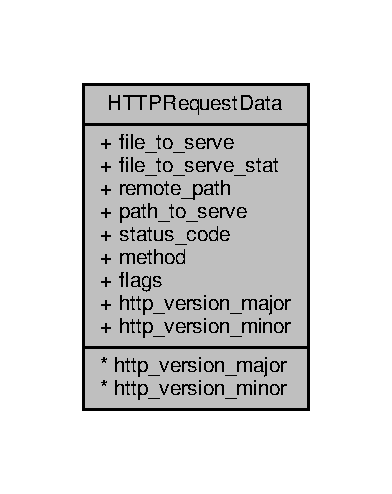
\includegraphics[width=188pt]{structHTTPRequestData__coll__graph}
\end{center}
\end{figure}
\subsection*{Campi}
\begin{DoxyCompactItemize}
\item 
F\+I\+L\+E $\ast$ \hyperlink{structHTTPRequestData_a52def24a4e2fefab7c723751b4ca5a7b}{file\+\_\+to\+\_\+serve}
\begin{DoxyCompactList}\small\item\em Il file da inviare, che può essere il file richiesto, nel caso in cui l\textquotesingle{}elaborazione della richiesta sia andata a buon fine, o una pagina di errore altrimenti. \end{DoxyCompactList}\item 
struct stat $\ast$ \hyperlink{structHTTPRequestData_acf9615119994e2784a395f3b5b80f710}{file\+\_\+to\+\_\+serve\+\_\+stat}
\begin{DoxyCompactList}\small\item\em Un puntatore al risultato di stat() eseguito sul file richiesto. \end{DoxyCompactList}\item 
char $\ast$ \hyperlink{structHTTPRequestData_a04c7c946a943f429f2529cf220076c26}{remote\+\_\+path}
\begin{DoxyCompactList}\small\item\em Il percorso come indicato nella richiesta. \end{DoxyCompactList}\item 
char $\ast$ \hyperlink{structHTTPRequestData_a71bcae8a8f14feb676826a6b8a76604e}{path\+\_\+to\+\_\+serve}
\begin{DoxyCompactList}\small\item\em Il percorso locale di file\+\_\+to\+\_\+serve. \end{DoxyCompactList}\item 
int \hyperlink{structHTTPRequestData_a47c202aa745d8a5eb2a5dc7cbc3087aa}{status\+\_\+code}
\begin{DoxyCompactList}\small\item\em Lo status code, come da inserire nella risposta, a cui ha dato origine l\textquotesingle{}elaborazione della richiesta. \end{DoxyCompactList}\item 
enum \hyperlink{httpheaders_8h_a837a089a977b319a11edfb8022d9e47d}{H\+T\+T\+P\+Method} \hyperlink{structHTTPRequestData_af309a4c6a758b62689eeb327b5e09737}{method}
\begin{DoxyCompactList}\small\item\em Un valore di H\+T\+T\+P\+Method rappresentante il metodo della richiesta. \end{DoxyCompactList}\item 
uint8\+\_\+t \hyperlink{structHTTPRequestData_ac3bd527bd3e00ce219bfa72dbaea2351}{flags}
\begin{DoxyCompactList}\small\item\em Bitmask rappresentante diverse informazioni sulla richiesta. \end{DoxyCompactList}\end{DoxyCompactItemize}
\begin{Indent}{\bf http\+\_\+version}\par
{\em La versione di H\+T\+T\+P, come indicata nella richiesta. }\begin{DoxyCompactItemize}
\item 
\hypertarget{structHTTPRequestData_ae0ec4135e692b7a72a0c218f80fcbe79}{}int {\bfseries http\+\_\+version\+\_\+major}\label{structHTTPRequestData_ae0ec4135e692b7a72a0c218f80fcbe79}

\item 
\hypertarget{structHTTPRequestData_ac0ecb1c39ad0d090ba95a3f90d52b424}{}int {\bfseries http\+\_\+version\+\_\+minor}\label{structHTTPRequestData_ac0ecb1c39ad0d090ba95a3f90d52b424}

\end{DoxyCompactItemize}
\end{Indent}


\subsection{Descrizione dettagliata}
Contiene informazioni su di una richiesta H\+T\+T\+P. 

Una volta elaborate, le informazioni su di una richiesta H\+T\+T\+P ricevuta dal server vengono raccolte in un\textquotesingle{}istanza di questa struttura. Una struttura \hyperlink{structHTTPRequestData}{H\+T\+T\+P\+Request\+Data} è restituita da \hyperlink{parse__request_8h_a7f6b46b8f33ebe0426d0d13b320f2927}{parse\+\_\+request()} dopo l\textquotesingle{}elaborazione a partire da una stringa, e può essere passata come parametro a \hyperlink{make__response_8h_adccd9b35824054b0c445e09f0731d706}{make\+\_\+response()} per elaborare la risposta del server. 

\subsection{Documentazione dei campi}
\hypertarget{structHTTPRequestData_a52def24a4e2fefab7c723751b4ca5a7b}{}\index{H\+T\+T\+P\+Request\+Data@{H\+T\+T\+P\+Request\+Data}!file\+\_\+to\+\_\+serve@{file\+\_\+to\+\_\+serve}}
\index{file\+\_\+to\+\_\+serve@{file\+\_\+to\+\_\+serve}!H\+T\+T\+P\+Request\+Data@{H\+T\+T\+P\+Request\+Data}}
\subsubsection[{file\+\_\+to\+\_\+serve}]{\setlength{\rightskip}{0pt plus 5cm}F\+I\+L\+E$\ast$ H\+T\+T\+P\+Request\+Data\+::file\+\_\+to\+\_\+serve}\label{structHTTPRequestData_a52def24a4e2fefab7c723751b4ca5a7b}


Il file da inviare, che può essere il file richiesto, nel caso in cui l\textquotesingle{}elaborazione della richiesta sia andata a buon fine, o una pagina di errore altrimenti. 

\hypertarget{structHTTPRequestData_acf9615119994e2784a395f3b5b80f710}{}\index{H\+T\+T\+P\+Request\+Data@{H\+T\+T\+P\+Request\+Data}!file\+\_\+to\+\_\+serve\+\_\+stat@{file\+\_\+to\+\_\+serve\+\_\+stat}}
\index{file\+\_\+to\+\_\+serve\+\_\+stat@{file\+\_\+to\+\_\+serve\+\_\+stat}!H\+T\+T\+P\+Request\+Data@{H\+T\+T\+P\+Request\+Data}}
\subsubsection[{file\+\_\+to\+\_\+serve\+\_\+stat}]{\setlength{\rightskip}{0pt plus 5cm}struct stat$\ast$ H\+T\+T\+P\+Request\+Data\+::file\+\_\+to\+\_\+serve\+\_\+stat}\label{structHTTPRequestData_acf9615119994e2784a395f3b5b80f710}


Un puntatore al risultato di stat() eseguito sul file richiesto. 

\hypertarget{structHTTPRequestData_ac3bd527bd3e00ce219bfa72dbaea2351}{}\index{H\+T\+T\+P\+Request\+Data@{H\+T\+T\+P\+Request\+Data}!flags@{flags}}
\index{flags@{flags}!H\+T\+T\+P\+Request\+Data@{H\+T\+T\+P\+Request\+Data}}
\subsubsection[{flags}]{\setlength{\rightskip}{0pt plus 5cm}uint8\+\_\+t H\+T\+T\+P\+Request\+Data\+::flags}\label{structHTTPRequestData_ac3bd527bd3e00ce219bfa72dbaea2351}


Bitmask rappresentante diverse informazioni sulla richiesta. 

\begin{DoxySeeAlso}{Si veda anche}
\hyperlink{httpdata_8h_a159dd434f3cab184e5fab8365ed494ec}{H\+T\+T\+P\+Request\+Data\+\_\+flags} 
\end{DoxySeeAlso}
\hypertarget{structHTTPRequestData_af309a4c6a758b62689eeb327b5e09737}{}\index{H\+T\+T\+P\+Request\+Data@{H\+T\+T\+P\+Request\+Data}!method@{method}}
\index{method@{method}!H\+T\+T\+P\+Request\+Data@{H\+T\+T\+P\+Request\+Data}}
\subsubsection[{method}]{\setlength{\rightskip}{0pt plus 5cm}enum {\bf H\+T\+T\+P\+Method} H\+T\+T\+P\+Request\+Data\+::method}\label{structHTTPRequestData_af309a4c6a758b62689eeb327b5e09737}


Un valore di H\+T\+T\+P\+Method rappresentante il metodo della richiesta. 

\hypertarget{structHTTPRequestData_a71bcae8a8f14feb676826a6b8a76604e}{}\index{H\+T\+T\+P\+Request\+Data@{H\+T\+T\+P\+Request\+Data}!path\+\_\+to\+\_\+serve@{path\+\_\+to\+\_\+serve}}
\index{path\+\_\+to\+\_\+serve@{path\+\_\+to\+\_\+serve}!H\+T\+T\+P\+Request\+Data@{H\+T\+T\+P\+Request\+Data}}
\subsubsection[{path\+\_\+to\+\_\+serve}]{\setlength{\rightskip}{0pt plus 5cm}char$\ast$ H\+T\+T\+P\+Request\+Data\+::path\+\_\+to\+\_\+serve}\label{structHTTPRequestData_a71bcae8a8f14feb676826a6b8a76604e}


Il percorso locale di file\+\_\+to\+\_\+serve. 

\hypertarget{structHTTPRequestData_a04c7c946a943f429f2529cf220076c26}{}\index{H\+T\+T\+P\+Request\+Data@{H\+T\+T\+P\+Request\+Data}!remote\+\_\+path@{remote\+\_\+path}}
\index{remote\+\_\+path@{remote\+\_\+path}!H\+T\+T\+P\+Request\+Data@{H\+T\+T\+P\+Request\+Data}}
\subsubsection[{remote\+\_\+path}]{\setlength{\rightskip}{0pt plus 5cm}char$\ast$ H\+T\+T\+P\+Request\+Data\+::remote\+\_\+path}\label{structHTTPRequestData_a04c7c946a943f429f2529cf220076c26}


Il percorso come indicato nella richiesta. 

\hypertarget{structHTTPRequestData_a47c202aa745d8a5eb2a5dc7cbc3087aa}{}\index{H\+T\+T\+P\+Request\+Data@{H\+T\+T\+P\+Request\+Data}!status\+\_\+code@{status\+\_\+code}}
\index{status\+\_\+code@{status\+\_\+code}!H\+T\+T\+P\+Request\+Data@{H\+T\+T\+P\+Request\+Data}}
\subsubsection[{status\+\_\+code}]{\setlength{\rightskip}{0pt plus 5cm}int H\+T\+T\+P\+Request\+Data\+::status\+\_\+code}\label{structHTTPRequestData_a47c202aa745d8a5eb2a5dc7cbc3087aa}


Lo status code, come da inserire nella risposta, a cui ha dato origine l\textquotesingle{}elaborazione della richiesta. 



La documentazione per questa struct è stata generata a partire dal seguente file\+:\begin{DoxyCompactItemize}
\item 
tnc/server/\hyperlink{httpdata_8h}{httpdata.\+h}\end{DoxyCompactItemize}

\hypertarget{structHTTPRequestHeader}{}\section{Riferimenti per la struct H\+T\+T\+P\+Request\+Header}
\label{structHTTPRequestHeader}\index{H\+T\+T\+P\+Request\+Header@{H\+T\+T\+P\+Request\+Header}}


Rappresenta un header di richiesta H\+T\+T\+P.  




{\ttfamily \#include $<$httpdata.\+h$>$}



Diagramma di collaborazione per H\+T\+T\+P\+Request\+Header\+:\nopagebreak
\begin{figure}[H]
\begin{center}
\leavevmode
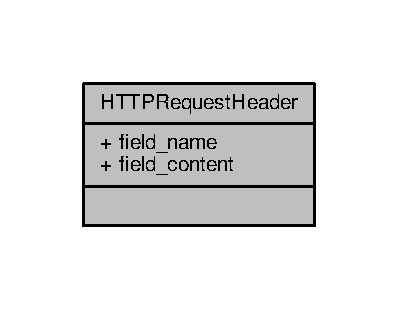
\includegraphics[width=191pt]{structHTTPRequestHeader__coll__graph}
\end{center}
\end{figure}
\subsection*{Campi}
\begin{DoxyCompactItemize}
\item 
char $\ast$ \hyperlink{structHTTPRequestHeader_a9455709e6aff8eb48c42866a1a674094}{field\+\_\+name}
\begin{DoxyCompactList}\small\item\em Il nome dell\textquotesingle{}header. \end{DoxyCompactList}\item 
char $\ast$ \hyperlink{structHTTPRequestHeader_a89cbb9f9651b0866bc4f0dbd37b5e435}{field\+\_\+content}
\begin{DoxyCompactList}\small\item\em Il valore dell\textquotesingle{}header. \end{DoxyCompactList}\end{DoxyCompactItemize}


\subsection{Descrizione dettagliata}
Rappresenta un header di richiesta H\+T\+T\+P. 



\subsection{Documentazione dei campi}
\hypertarget{structHTTPRequestHeader_a89cbb9f9651b0866bc4f0dbd37b5e435}{}\index{H\+T\+T\+P\+Request\+Header@{H\+T\+T\+P\+Request\+Header}!field\+\_\+content@{field\+\_\+content}}
\index{field\+\_\+content@{field\+\_\+content}!H\+T\+T\+P\+Request\+Header@{H\+T\+T\+P\+Request\+Header}}
\subsubsection[{field\+\_\+content}]{\setlength{\rightskip}{0pt plus 5cm}char$\ast$ H\+T\+T\+P\+Request\+Header\+::field\+\_\+content}\label{structHTTPRequestHeader_a89cbb9f9651b0866bc4f0dbd37b5e435}


Il valore dell\textquotesingle{}header. 

\hypertarget{structHTTPRequestHeader_a9455709e6aff8eb48c42866a1a674094}{}\index{H\+T\+T\+P\+Request\+Header@{H\+T\+T\+P\+Request\+Header}!field\+\_\+name@{field\+\_\+name}}
\index{field\+\_\+name@{field\+\_\+name}!H\+T\+T\+P\+Request\+Header@{H\+T\+T\+P\+Request\+Header}}
\subsubsection[{field\+\_\+name}]{\setlength{\rightskip}{0pt plus 5cm}char$\ast$ H\+T\+T\+P\+Request\+Header\+::field\+\_\+name}\label{structHTTPRequestHeader_a9455709e6aff8eb48c42866a1a674094}


Il nome dell\textquotesingle{}header. 



La documentazione per questa struct è stata generata a partire dal seguente file\+:\begin{DoxyCompactItemize}
\item 
tnc/server/\hyperlink{httpdata_8h}{httpdata.\+h}\end{DoxyCompactItemize}

\hypertarget{structHTTPResponseData}{}\section{Riferimenti per la struct H\+T\+T\+P\+Response\+Data}
\label{structHTTPResponseData}\index{H\+T\+T\+P\+Response\+Data@{H\+T\+T\+P\+Response\+Data}}


Diagramma di collaborazione per H\+T\+T\+P\+Response\+Data\+:\nopagebreak
\begin{figure}[H]
\begin{center}
\leavevmode
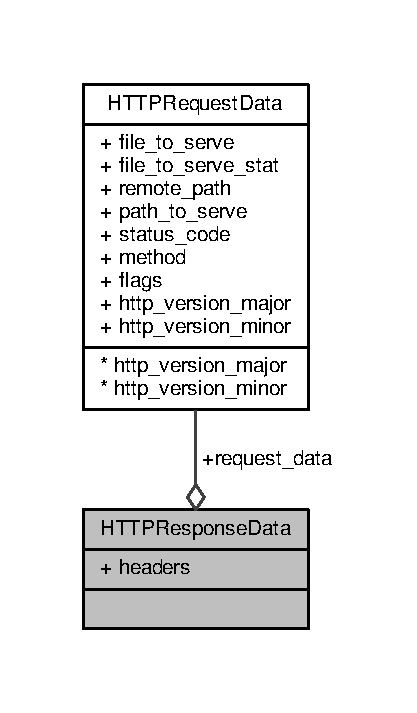
\includegraphics[width=200pt]{structHTTPResponseData__coll__graph}
\end{center}
\end{figure}
\subsection*{Campi}
\begin{DoxyCompactItemize}
\item 
\hypertarget{structHTTPResponseData_a2ea29f58aa5a67164dcdaa8cc9300340}{}const \hyperlink{structHTTPRequestData}{H\+T\+T\+P\+Request\+Data} $\ast$ {\bfseries request\+\_\+data}\label{structHTTPResponseData_a2ea29f58aa5a67164dcdaa8cc9300340}

\item 
\hypertarget{structHTTPResponseData_ab12d3e6ec05acade8e26c354a15e1d98}{}T\+N\+C\+List {\bfseries headers}\label{structHTTPResponseData_ab12d3e6ec05acade8e26c354a15e1d98}

\end{DoxyCompactItemize}


La documentazione per questa struct è stata generata a partire dal seguente file\+:\begin{DoxyCompactItemize}
\item 
tnc/server/\hyperlink{httpdata_8h}{httpdata.\+h}\end{DoxyCompactItemize}

\hypertarget{structTNCJob}{}\section{Riferimenti per la struct T\+N\+C\+Job}
\label{structTNCJob}\index{T\+N\+C\+Job@{T\+N\+C\+Job}}


Diagramma di collaborazione per T\+N\+C\+Job\+:\nopagebreak
\begin{figure}[H]
\begin{center}
\leavevmode
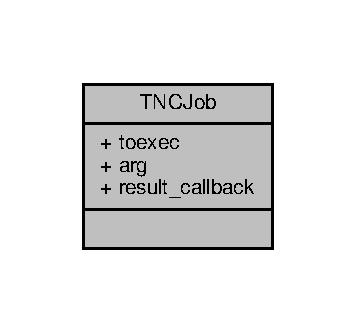
\includegraphics[width=171pt]{structTNCJob__coll__graph}
\end{center}
\end{figure}
\subsection*{Campi}
\begin{DoxyCompactItemize}
\item 
\hypertarget{structTNCJob_a9700d43a243f74081b3157d32d86bde2}{}\hyperlink{functiontypes_8h_ab55be5b67db12c27273a3598b1be3d8a}{T\+N\+C\+Function} {\bfseries toexec}\label{structTNCJob_a9700d43a243f74081b3157d32d86bde2}

\item 
\hypertarget{structTNCJob_af68654e56326315994369f9652f26deb}{}void $\ast$ {\bfseries arg}\label{structTNCJob_af68654e56326315994369f9652f26deb}

\item 
\hypertarget{structTNCJob_a561ecf6ddfc315c7307d10325c5777c5}{}\hyperlink{functiontypes_8h_a78b4c663dde4687b8cddd1ca6031cadb}{T\+N\+C\+Consumer} {\bfseries result\+\_\+callback}\label{structTNCJob_a561ecf6ddfc315c7307d10325c5777c5}

\end{DoxyCompactItemize}


La documentazione per questa struct è stata generata a partire dal seguente file\+:\begin{DoxyCompactItemize}
\item 
tnc/core/\hyperlink{fixedthreadpool_8h}{fixedthreadpool.\+h}\end{DoxyCompactItemize}

\chapter{Documentazione dei file}
\hypertarget{core_2error_8h}{}\section{Riferimenti per il file tnc/core/error.h}
\label{core_2error_8h}\index{tnc/core/error.\+h@{tnc/core/error.\+h}}


Contiene i codici di errore restituiti dalle funzioni.  


Questo grafo mostra quali altri file includono direttamente o indirettamente questo file\+:\nopagebreak
\begin{figure}[H]
\begin{center}
\leavevmode
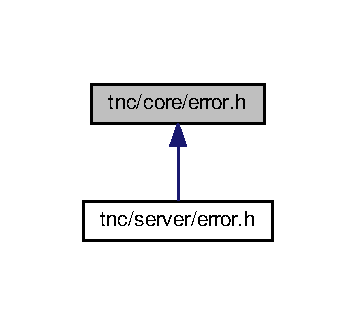
\includegraphics[width=171pt]{core_2error_8h__dep__incl}
\end{center}
\end{figure}
\subsection*{Tipi enumerati (enum)}
\begin{DoxyCompactItemize}
\item 
enum \hyperlink{core_2error_8h_a79628632b882851eaec13e771163bdde}{T\+N\+C\+Error} \{ \hyperlink{core_2error_8h_a79628632b882851eaec13e771163bddeaff870e40cb81baab0eadd0890a94a5ac}{T\+N\+C\+Error\+\_\+good} = 0, 
\hyperlink{core_2error_8h_a79628632b882851eaec13e771163bddea7cdfd5b81b1a0fb6e53fb928963ec2ad}{T\+N\+C\+Error\+\_\+failed\+\_\+alloc} = 1, 
\hyperlink{core_2error_8h_a79628632b882851eaec13e771163bddea201f978617f9c2746a7fbf97ee1b671b}{T\+N\+C\+Error\+\_\+thread\+\_\+start\+\_\+failed}, 
\hyperlink{core_2error_8h_a79628632b882851eaec13e771163bddea220fda8de0e7697ea743f277fc92289b}{T\+N\+C\+Error\+\_\+module\+\_\+defined}
 \}
\end{DoxyCompactItemize}


\subsection{Descrizione dettagliata}
Contiene i codici di errore restituiti dalle funzioni. 



\subsection{Documentazione dei tipi enumerati}
\hypertarget{core_2error_8h_a79628632b882851eaec13e771163bdde}{}\index{core/error.\+h@{core/error.\+h}!T\+N\+C\+Error@{T\+N\+C\+Error}}
\index{T\+N\+C\+Error@{T\+N\+C\+Error}!core/error.\+h@{core/error.\+h}}
\subsubsection[{T\+N\+C\+Error}]{\setlength{\rightskip}{0pt plus 5cm}enum {\bf T\+N\+C\+Error}}\label{core_2error_8h_a79628632b882851eaec13e771163bdde}
\begin{Desc}
\item[Valori del tipo enumerato]\par
\begin{description}
\index{T\+N\+C\+Error\+\_\+good@{T\+N\+C\+Error\+\_\+good}!core/error.\+h@{core/error.\+h}}\index{core/error.\+h@{core/error.\+h}!T\+N\+C\+Error\+\_\+good@{T\+N\+C\+Error\+\_\+good}}\item[{\em 
\hypertarget{core_2error_8h_a79628632b882851eaec13e771163bddeaff870e40cb81baab0eadd0890a94a5ac}{}T\+N\+C\+Error\+\_\+good\label{core_2error_8h_a79628632b882851eaec13e771163bddeaff870e40cb81baab0eadd0890a94a5ac}
}]La funzione è terminata con esito positivo. \index{T\+N\+C\+Error\+\_\+failed\+\_\+alloc@{T\+N\+C\+Error\+\_\+failed\+\_\+alloc}!core/error.\+h@{core/error.\+h}}\index{core/error.\+h@{core/error.\+h}!T\+N\+C\+Error\+\_\+failed\+\_\+alloc@{T\+N\+C\+Error\+\_\+failed\+\_\+alloc}}\item[{\em 
\hypertarget{core_2error_8h_a79628632b882851eaec13e771163bddea7cdfd5b81b1a0fb6e53fb928963ec2ad}{}T\+N\+C\+Error\+\_\+failed\+\_\+alloc\label{core_2error_8h_a79628632b882851eaec13e771163bddea7cdfd5b81b1a0fb6e53fb928963ec2ad}
}]Un\textquotesingle{}allocazione di memoria necessaria per l\textquotesingle{}esecuzione della funzione è fallita. \index{T\+N\+C\+Error\+\_\+thread\+\_\+start\+\_\+failed@{T\+N\+C\+Error\+\_\+thread\+\_\+start\+\_\+failed}!core/error.\+h@{core/error.\+h}}\index{core/error.\+h@{core/error.\+h}!T\+N\+C\+Error\+\_\+thread\+\_\+start\+\_\+failed@{T\+N\+C\+Error\+\_\+thread\+\_\+start\+\_\+failed}}\item[{\em 
\hypertarget{core_2error_8h_a79628632b882851eaec13e771163bddea201f978617f9c2746a7fbf97ee1b671b}{}T\+N\+C\+Error\+\_\+thread\+\_\+start\+\_\+failed\label{core_2error_8h_a79628632b882851eaec13e771163bddea201f978617f9c2746a7fbf97ee1b671b}
}]L\textquotesingle{}avvio di un thread nella funzione è fallito. \index{T\+N\+C\+Error\+\_\+module\+\_\+defined@{T\+N\+C\+Error\+\_\+module\+\_\+defined}!core/error.\+h@{core/error.\+h}}\index{core/error.\+h@{core/error.\+h}!T\+N\+C\+Error\+\_\+module\+\_\+defined@{T\+N\+C\+Error\+\_\+module\+\_\+defined}}\item[{\em 
\hypertarget{core_2error_8h_a79628632b882851eaec13e771163bddea220fda8de0e7697ea743f277fc92289b}{}T\+N\+C\+Error\+\_\+module\+\_\+defined\label{core_2error_8h_a79628632b882851eaec13e771163bddea220fda8de0e7697ea743f277fc92289b}
}]Indica l\textquotesingle{}inizio dei valori di errori dipendenti dal modulo. \end{description}
\end{Desc}

\hypertarget{server_2error_8h}{}\section{Riferimenti per il file tnc/server/error.h}
\label{server_2error_8h}\index{tnc/server/error.\+h@{tnc/server/error.\+h}}


Contiene codici di errore restituiti dalle funzioni relative al server.  


{\ttfamily \#include \char`\"{}tnc/core/error.\+h\char`\"{}}\\*
Grafo delle dipendenze di inclusione per error.\+h\+:\nopagebreak
\begin{figure}[H]
\begin{center}
\leavevmode
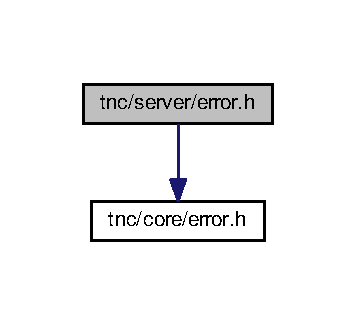
\includegraphics[width=171pt]{server_2error_8h__incl}
\end{center}
\end{figure}
\subsection*{Tipi enumerati (enum)}
\begin{DoxyCompactItemize}
\item 
enum \hyperlink{server_2error_8h_a1d5b92b34fed183ee9b57f13a77fd81b}{T\+N\+C\+Server\+Error} \{ \\*
\hyperlink{server_2error_8h_a1d5b92b34fed183ee9b57f13a77fd81ba7e1aa806d11853faeaa70eecca881d44}{T\+N\+C\+Server\+Error\+\_\+invalid\+\_\+path} = T\+N\+C\+Error\+\_\+module\+\_\+defined, 
\hyperlink{server_2error_8h_a1d5b92b34fed183ee9b57f13a77fd81ba7263758bd4daa9a19f63fa388726ebb1}{T\+N\+C\+Server\+Error\+\_\+connection\+\_\+failed}, 
\hyperlink{server_2error_8h_a1d5b92b34fed183ee9b57f13a77fd81baf8e7ed9e4375af5f7231aa97354ff79f}{T\+N\+C\+Server\+Error\+\_\+fn\+\_\+getaddrinfo\+\_\+failed}, 
\hyperlink{server_2error_8h_a1d5b92b34fed183ee9b57f13a77fd81ba08bef902bf386dca35be7c9ae2bfe99a}{T\+N\+C\+Server\+Error\+\_\+fn\+\_\+socket\+\_\+failed}, 
\\*
\hyperlink{server_2error_8h_a1d5b92b34fed183ee9b57f13a77fd81ba7f98ce8ed64bc3d43bcefbdacc7519b7}{T\+N\+C\+Server\+Error\+\_\+fn\+\_\+setsockopt\+\_\+failed}, 
\hyperlink{server_2error_8h_a1d5b92b34fed183ee9b57f13a77fd81ba8bebf851afeb7ae21edcb645537496e7}{T\+N\+C\+Server\+Error\+\_\+fn\+\_\+bind\+\_\+failed}
 \}
\begin{DoxyCompactList}\small\item\em Codici di errore restituiti dalle funzioni relative al server. \end{DoxyCompactList}\end{DoxyCompactItemize}


\subsection{Descrizione dettagliata}
Contiene codici di errore restituiti dalle funzioni relative al server. 



\subsection{Documentazione dei tipi enumerati}
\hypertarget{server_2error_8h_a1d5b92b34fed183ee9b57f13a77fd81b}{}\index{server/error.\+h@{server/error.\+h}!T\+N\+C\+Server\+Error@{T\+N\+C\+Server\+Error}}
\index{T\+N\+C\+Server\+Error@{T\+N\+C\+Server\+Error}!server/error.\+h@{server/error.\+h}}
\subsubsection[{T\+N\+C\+Server\+Error}]{\setlength{\rightskip}{0pt plus 5cm}enum {\bf T\+N\+C\+Server\+Error}}\label{server_2error_8h_a1d5b92b34fed183ee9b57f13a77fd81b}


Codici di errore restituiti dalle funzioni relative al server. 

\begin{Desc}
\item[Valori del tipo enumerato]\par
\begin{description}
\index{T\+N\+C\+Server\+Error\+\_\+invalid\+\_\+path@{T\+N\+C\+Server\+Error\+\_\+invalid\+\_\+path}!server/error.\+h@{server/error.\+h}}\index{server/error.\+h@{server/error.\+h}!T\+N\+C\+Server\+Error\+\_\+invalid\+\_\+path@{T\+N\+C\+Server\+Error\+\_\+invalid\+\_\+path}}\item[{\em 
\hypertarget{server_2error_8h_a1d5b92b34fed183ee9b57f13a77fd81ba7e1aa806d11853faeaa70eecca881d44}{}T\+N\+C\+Server\+Error\+\_\+invalid\+\_\+path\label{server_2error_8h_a1d5b92b34fed183ee9b57f13a77fd81ba7e1aa806d11853faeaa70eecca881d44}
}]Il percorso indicato come parametro non è valido. \index{T\+N\+C\+Server\+Error\+\_\+connection\+\_\+failed@{T\+N\+C\+Server\+Error\+\_\+connection\+\_\+failed}!server/error.\+h@{server/error.\+h}}\index{server/error.\+h@{server/error.\+h}!T\+N\+C\+Server\+Error\+\_\+connection\+\_\+failed@{T\+N\+C\+Server\+Error\+\_\+connection\+\_\+failed}}\item[{\em 
\hypertarget{server_2error_8h_a1d5b92b34fed183ee9b57f13a77fd81ba7263758bd4daa9a19f63fa388726ebb1}{}T\+N\+C\+Server\+Error\+\_\+connection\+\_\+failed\label{server_2error_8h_a1d5b92b34fed183ee9b57f13a77fd81ba7263758bd4daa9a19f63fa388726ebb1}
}]La connessione non è andata a buon fine. \index{T\+N\+C\+Server\+Error\+\_\+fn\+\_\+getaddrinfo\+\_\+failed@{T\+N\+C\+Server\+Error\+\_\+fn\+\_\+getaddrinfo\+\_\+failed}!server/error.\+h@{server/error.\+h}}\index{server/error.\+h@{server/error.\+h}!T\+N\+C\+Server\+Error\+\_\+fn\+\_\+getaddrinfo\+\_\+failed@{T\+N\+C\+Server\+Error\+\_\+fn\+\_\+getaddrinfo\+\_\+failed}}\item[{\em 
\hypertarget{server_2error_8h_a1d5b92b34fed183ee9b57f13a77fd81baf8e7ed9e4375af5f7231aa97354ff79f}{}T\+N\+C\+Server\+Error\+\_\+fn\+\_\+getaddrinfo\+\_\+failed\label{server_2error_8h_a1d5b92b34fed183ee9b57f13a77fd81baf8e7ed9e4375af5f7231aa97354ff79f}
}]La risoluzione D\+N\+S tramite la funzione getaddrinfo() non è andata a buon fine. \index{T\+N\+C\+Server\+Error\+\_\+fn\+\_\+socket\+\_\+failed@{T\+N\+C\+Server\+Error\+\_\+fn\+\_\+socket\+\_\+failed}!server/error.\+h@{server/error.\+h}}\index{server/error.\+h@{server/error.\+h}!T\+N\+C\+Server\+Error\+\_\+fn\+\_\+socket\+\_\+failed@{T\+N\+C\+Server\+Error\+\_\+fn\+\_\+socket\+\_\+failed}}\item[{\em 
\hypertarget{server_2error_8h_a1d5b92b34fed183ee9b57f13a77fd81ba08bef902bf386dca35be7c9ae2bfe99a}{}T\+N\+C\+Server\+Error\+\_\+fn\+\_\+socket\+\_\+failed\label{server_2error_8h_a1d5b92b34fed183ee9b57f13a77fd81ba08bef902bf386dca35be7c9ae2bfe99a}
}]La funzione socket() ha restituito un errore. \index{T\+N\+C\+Server\+Error\+\_\+fn\+\_\+setsockopt\+\_\+failed@{T\+N\+C\+Server\+Error\+\_\+fn\+\_\+setsockopt\+\_\+failed}!server/error.\+h@{server/error.\+h}}\index{server/error.\+h@{server/error.\+h}!T\+N\+C\+Server\+Error\+\_\+fn\+\_\+setsockopt\+\_\+failed@{T\+N\+C\+Server\+Error\+\_\+fn\+\_\+setsockopt\+\_\+failed}}\item[{\em 
\hypertarget{server_2error_8h_a1d5b92b34fed183ee9b57f13a77fd81ba7f98ce8ed64bc3d43bcefbdacc7519b7}{}T\+N\+C\+Server\+Error\+\_\+fn\+\_\+setsockopt\+\_\+failed\label{server_2error_8h_a1d5b92b34fed183ee9b57f13a77fd81ba7f98ce8ed64bc3d43bcefbdacc7519b7}
}]La funzione setsockopt() ha restituito un errore. \index{T\+N\+C\+Server\+Error\+\_\+fn\+\_\+bind\+\_\+failed@{T\+N\+C\+Server\+Error\+\_\+fn\+\_\+bind\+\_\+failed}!server/error.\+h@{server/error.\+h}}\index{server/error.\+h@{server/error.\+h}!T\+N\+C\+Server\+Error\+\_\+fn\+\_\+bind\+\_\+failed@{T\+N\+C\+Server\+Error\+\_\+fn\+\_\+bind\+\_\+failed}}\item[{\em 
\hypertarget{server_2error_8h_a1d5b92b34fed183ee9b57f13a77fd81ba8bebf851afeb7ae21edcb645537496e7}{}T\+N\+C\+Server\+Error\+\_\+fn\+\_\+bind\+\_\+failed\label{server_2error_8h_a1d5b92b34fed183ee9b57f13a77fd81ba8bebf851afeb7ae21edcb645537496e7}
}]La funzione bind() ha restituito un errore. \end{description}
\end{Desc}

\hypertarget{fixedthreadpool_8h}{}\section{Riferimenti per il file tnc/core/fixedthreadpool.h}
\label{fixedthreadpool_8h}\index{tnc/core/fixedthreadpool.\+h@{tnc/core/fixedthreadpool.\+h}}


Contiene l\textquotesingle{}interfaccia per i threadpool.  


{\ttfamily \#include $<$stdlib.\+h$>$}\\*
{\ttfamily \#include \char`\"{}functiontypes.\+h\char`\"{}}\\*
Grafo delle dipendenze di inclusione per fixedthreadpool.\+h\+:\nopagebreak
\begin{figure}[H]
\begin{center}
\leavevmode
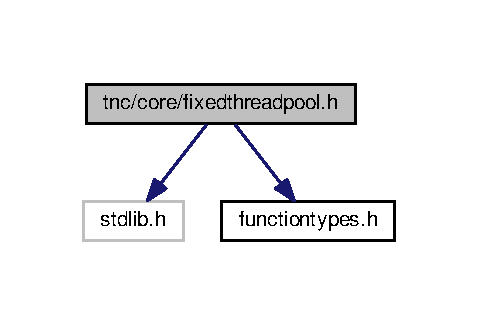
\includegraphics[width=230pt]{fixedthreadpool_8h__incl}
\end{center}
\end{figure}
Questo grafo mostra quali altri file includono direttamente o indirettamente questo file\+:
\nopagebreak
\begin{figure}[H]
\begin{center}
\leavevmode
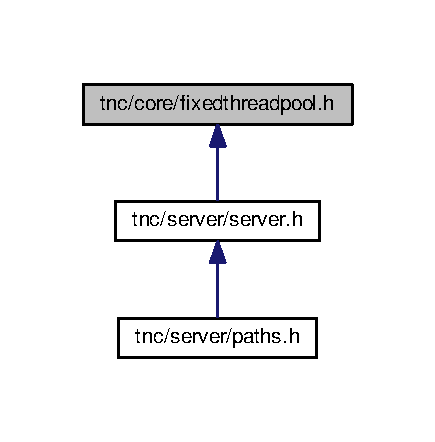
\includegraphics[width=209pt]{fixedthreadpool_8h__dep__incl}
\end{center}
\end{figure}
\subsection*{Strutture dati}
\begin{DoxyCompactItemize}
\item 
struct \hyperlink{structTNCJob}{T\+N\+C\+Job}
\end{DoxyCompactItemize}
\subsection*{Tipi enumerati (enum)}
\begin{DoxyCompactItemize}
\item 
\hypertarget{fixedthreadpool_8h_a07df799d1391cfaf2f15dd1fb76d1580}{}enum {\bfseries T\+N\+C\+Fixed\+Thread\+Pool\+\_\+shutdown\+\_\+flags} \{ {\bfseries T\+N\+C\+Thread\+Pool\+\_\+shutdown\+\_\+now} = 1, 
{\bfseries T\+N\+C\+Thread\+Pool\+\_\+shutdown\+\_\+finish\+\_\+pending}
 \}\label{fixedthreadpool_8h_a07df799d1391cfaf2f15dd1fb76d1580}

\item 
\hypertarget{fixedthreadpool_8h_aa98f20da9b8b04c23f65df0ad4938cbd}{}enum {\bfseries T\+N\+C\+Fixed\+Thread\+Pool\+\_\+wait} \{ {\bfseries T\+N\+C\+Thread\+Pool\+\_\+wait\+\_\+yes} = 1, 
{\bfseries T\+N\+C\+Thread\+Pool\+\_\+wait\+\_\+no}
 \}\label{fixedthreadpool_8h_aa98f20da9b8b04c23f65df0ad4938cbd}

\end{DoxyCompactItemize}
\subsection*{Funzioni}
\begin{DoxyCompactItemize}
\item 
T\+N\+C\+Fixed\+Thread\+Pool \hyperlink{fixedthreadpool_8h_a1c95e2e20301036bd8fe65c716c83022}{T\+N\+C\+Fixed\+Thread\+Pool\+\_\+new} (size\+\_\+t threads)
\begin{DoxyCompactList}\small\item\em Crea un threadpool. \end{DoxyCompactList}\item 
int \hyperlink{fixedthreadpool_8h_a47a491dfca90579d121f8412f20d58c0}{T\+N\+C\+Fixed\+Thread\+Pool\+\_\+start} (T\+N\+C\+Fixed\+Thread\+Pool self)
\begin{DoxyCompactList}\small\item\em Avvia un threadpool. \end{DoxyCompactList}\item 
void \hyperlink{fixedthreadpool_8h_acfe0d05944c3845441419ec2ad1eb61f}{T\+N\+C\+Fixed\+Thread\+Pool\+\_\+shutdown} (T\+N\+C\+Fixed\+Thread\+Pool self, enum T\+N\+C\+Fixed\+Thread\+Pool\+\_\+shutdown\+\_\+flags mode, enum T\+N\+C\+Fixed\+Thread\+Pool\+\_\+wait wait)
\begin{DoxyCompactList}\small\item\em Termina i worker di un threadpool. \end{DoxyCompactList}\item 
int \hyperlink{fixedthreadpool_8h_a06aa0b55a7af15a28e611b67121f6947}{T\+N\+C\+Fixed\+Thread\+Pool\+\_\+enqueue} (T\+N\+C\+Fixed\+Thread\+Pool self, \hyperlink{structTNCJob}{T\+N\+C\+Job} $\ast$job)
\begin{DoxyCompactList}\small\item\em Accoda un nuovo job alla coda. \end{DoxyCompactList}\item 
int \hyperlink{fixedthreadpool_8h_af2dbf489ca7d90b5e4074b15799a28ab}{T\+N\+C\+Fixed\+Thread\+Pool\+\_\+do\+\_\+next} (T\+N\+C\+Fixed\+Thread\+Pool self, \hyperlink{structTNCJob}{T\+N\+C\+Job} $\ast$job)
\begin{DoxyCompactList}\small\item\em Mette un nuovo job di fronte coda. \end{DoxyCompactList}\item 
void \hyperlink{fixedthreadpool_8h_a51de2e4133de8f60bcfe680b8ac3c4a9}{T\+N\+C\+Fixed\+Thread\+Pool\+\_\+destroy} (T\+N\+C\+Fixed\+Thread\+Pool self)
\begin{DoxyCompactList}\small\item\em Distrugge (dealloca) un T\+N\+C\+Fixed\+Thread\+Pool. \end{DoxyCompactList}\end{DoxyCompactItemize}


\subsection{Descrizione dettagliata}
Contiene l\textquotesingle{}interfaccia per i threadpool. 



\subsection{Documentazione delle funzioni}
\hypertarget{fixedthreadpool_8h_a51de2e4133de8f60bcfe680b8ac3c4a9}{}\index{fixedthreadpool.\+h@{fixedthreadpool.\+h}!T\+N\+C\+Fixed\+Thread\+Pool\+\_\+destroy@{T\+N\+C\+Fixed\+Thread\+Pool\+\_\+destroy}}
\index{T\+N\+C\+Fixed\+Thread\+Pool\+\_\+destroy@{T\+N\+C\+Fixed\+Thread\+Pool\+\_\+destroy}!fixedthreadpool.\+h@{fixedthreadpool.\+h}}
\subsubsection[{T\+N\+C\+Fixed\+Thread\+Pool\+\_\+destroy}]{\setlength{\rightskip}{0pt plus 5cm}void T\+N\+C\+Fixed\+Thread\+Pool\+\_\+destroy (
\begin{DoxyParamCaption}
\item[{T\+N\+C\+Fixed\+Thread\+Pool}]{self}
\end{DoxyParamCaption}
)}\label{fixedthreadpool_8h_a51de2e4133de8f60bcfe680b8ac3c4a9}


Distrugge (dealloca) un T\+N\+C\+Fixed\+Thread\+Pool. 

\hypertarget{fixedthreadpool_8h_af2dbf489ca7d90b5e4074b15799a28ab}{}\index{fixedthreadpool.\+h@{fixedthreadpool.\+h}!T\+N\+C\+Fixed\+Thread\+Pool\+\_\+do\+\_\+next@{T\+N\+C\+Fixed\+Thread\+Pool\+\_\+do\+\_\+next}}
\index{T\+N\+C\+Fixed\+Thread\+Pool\+\_\+do\+\_\+next@{T\+N\+C\+Fixed\+Thread\+Pool\+\_\+do\+\_\+next}!fixedthreadpool.\+h@{fixedthreadpool.\+h}}
\subsubsection[{T\+N\+C\+Fixed\+Thread\+Pool\+\_\+do\+\_\+next}]{\setlength{\rightskip}{0pt plus 5cm}int T\+N\+C\+Fixed\+Thread\+Pool\+\_\+do\+\_\+next (
\begin{DoxyParamCaption}
\item[{T\+N\+C\+Fixed\+Thread\+Pool}]{self, }
\item[{{\bf T\+N\+C\+Job} $\ast$}]{job}
\end{DoxyParamCaption}
)}\label{fixedthreadpool_8h_af2dbf489ca7d90b5e4074b15799a28ab}


Mette un nuovo job di fronte coda. 

\hypertarget{fixedthreadpool_8h_a06aa0b55a7af15a28e611b67121f6947}{}\index{fixedthreadpool.\+h@{fixedthreadpool.\+h}!T\+N\+C\+Fixed\+Thread\+Pool\+\_\+enqueue@{T\+N\+C\+Fixed\+Thread\+Pool\+\_\+enqueue}}
\index{T\+N\+C\+Fixed\+Thread\+Pool\+\_\+enqueue@{T\+N\+C\+Fixed\+Thread\+Pool\+\_\+enqueue}!fixedthreadpool.\+h@{fixedthreadpool.\+h}}
\subsubsection[{T\+N\+C\+Fixed\+Thread\+Pool\+\_\+enqueue}]{\setlength{\rightskip}{0pt plus 5cm}int T\+N\+C\+Fixed\+Thread\+Pool\+\_\+enqueue (
\begin{DoxyParamCaption}
\item[{T\+N\+C\+Fixed\+Thread\+Pool}]{self, }
\item[{{\bf T\+N\+C\+Job} $\ast$}]{job}
\end{DoxyParamCaption}
)}\label{fixedthreadpool_8h_a06aa0b55a7af15a28e611b67121f6947}


Accoda un nuovo job alla coda. 

\hypertarget{fixedthreadpool_8h_a1c95e2e20301036bd8fe65c716c83022}{}\index{fixedthreadpool.\+h@{fixedthreadpool.\+h}!T\+N\+C\+Fixed\+Thread\+Pool\+\_\+new@{T\+N\+C\+Fixed\+Thread\+Pool\+\_\+new}}
\index{T\+N\+C\+Fixed\+Thread\+Pool\+\_\+new@{T\+N\+C\+Fixed\+Thread\+Pool\+\_\+new}!fixedthreadpool.\+h@{fixedthreadpool.\+h}}
\subsubsection[{T\+N\+C\+Fixed\+Thread\+Pool\+\_\+new}]{\setlength{\rightskip}{0pt plus 5cm}T\+N\+C\+Fixed\+Thread\+Pool T\+N\+C\+Fixed\+Thread\+Pool\+\_\+new (
\begin{DoxyParamCaption}
\item[{size\+\_\+t}]{threads}
\end{DoxyParamCaption}
)}\label{fixedthreadpool_8h_a1c95e2e20301036bd8fe65c716c83022}


Crea un threadpool. 


\begin{DoxyParams}{Parametri}
{\em threads} & Il numero di worker nel pool.\\
\hline
\end{DoxyParams}
\begin{DoxyReturn}{Restituisce}
Un T\+N\+C\+Fixed\+Thread\+Pool se l\textquotesingle{}operazione va a buon fine, N\+U\+L\+L altrimenti. 
\end{DoxyReturn}
\hypertarget{fixedthreadpool_8h_acfe0d05944c3845441419ec2ad1eb61f}{}\index{fixedthreadpool.\+h@{fixedthreadpool.\+h}!T\+N\+C\+Fixed\+Thread\+Pool\+\_\+shutdown@{T\+N\+C\+Fixed\+Thread\+Pool\+\_\+shutdown}}
\index{T\+N\+C\+Fixed\+Thread\+Pool\+\_\+shutdown@{T\+N\+C\+Fixed\+Thread\+Pool\+\_\+shutdown}!fixedthreadpool.\+h@{fixedthreadpool.\+h}}
\subsubsection[{T\+N\+C\+Fixed\+Thread\+Pool\+\_\+shutdown}]{\setlength{\rightskip}{0pt plus 5cm}void T\+N\+C\+Fixed\+Thread\+Pool\+\_\+shutdown (
\begin{DoxyParamCaption}
\item[{T\+N\+C\+Fixed\+Thread\+Pool}]{self, }
\item[{enum T\+N\+C\+Fixed\+Thread\+Pool\+\_\+shutdown\+\_\+flags}]{mode, }
\item[{enum T\+N\+C\+Fixed\+Thread\+Pool\+\_\+wait}]{wait}
\end{DoxyParamCaption}
)}\label{fixedthreadpool_8h_acfe0d05944c3845441419ec2ad1eb61f}


Termina i worker di un threadpool. 


\begin{DoxyParams}{Parametri}
{\em self} & Il threadpool su cui si vuole operare.\\
\hline
{\em mode} & Parametro che indica la modalità di spegnimento. Se settato su T\+N\+C\+Thread\+Pool\+\_\+shutdown\+\_\+now, lo spegnimento non attenderà il termine dei job ancora nella coda. Se settato su T\+N\+C\+Thread\+Pool\+\_\+shutdown\+\_\+finish\+\_\+pending lo spegnimento avverrà al termine dei job ancora rimasti nella coda.\\
\hline
{\em wait} & Parametro che indica se la chiamata a shutdown blocca l\textquotesingle{}esecuzione. Se settato a T\+N\+C\+Thread\+Pool\+\_\+wait\+\_\+yes, la chiamata a shutdown blocca l\textquotesingle{}esecuzione fino al termine di tutti i thread. Se settato a T\+N\+C\+Thread\+Pool\+\_\+wait\+\_\+no, la chiamata a shutdown restituisce prima del termine dell\textquotesingle{}esecuzione dei thread rimanenti. \\
\hline
\end{DoxyParams}
\hypertarget{fixedthreadpool_8h_a47a491dfca90579d121f8412f20d58c0}{}\index{fixedthreadpool.\+h@{fixedthreadpool.\+h}!T\+N\+C\+Fixed\+Thread\+Pool\+\_\+start@{T\+N\+C\+Fixed\+Thread\+Pool\+\_\+start}}
\index{T\+N\+C\+Fixed\+Thread\+Pool\+\_\+start@{T\+N\+C\+Fixed\+Thread\+Pool\+\_\+start}!fixedthreadpool.\+h@{fixedthreadpool.\+h}}
\subsubsection[{T\+N\+C\+Fixed\+Thread\+Pool\+\_\+start}]{\setlength{\rightskip}{0pt plus 5cm}int T\+N\+C\+Fixed\+Thread\+Pool\+\_\+start (
\begin{DoxyParamCaption}
\item[{T\+N\+C\+Fixed\+Thread\+Pool}]{self}
\end{DoxyParamCaption}
)}\label{fixedthreadpool_8h_a47a491dfca90579d121f8412f20d58c0}


Avvia un threadpool. 


\begin{DoxyParams}{Parametri}
{\em self} & Il threadpool da avviare.\\
\hline
\end{DoxyParams}
\begin{DoxyReturn}{Restituisce}
Un codice di errore. I codici di errore si possono trovare nell\textquotesingle{}header error.\+h. 
\end{DoxyReturn}

\hypertarget{functiontypes_8h}{}\section{Riferimenti per il file tnc/core/functiontypes.h}
\label{functiontypes_8h}\index{tnc/core/functiontypes.\+h@{tnc/core/functiontypes.\+h}}


Contiene alias a tipo di puntatore a funzione.  


Questo grafo mostra quali altri file includono direttamente o indirettamente questo file\+:
\nopagebreak
\begin{figure}[H]
\begin{center}
\leavevmode
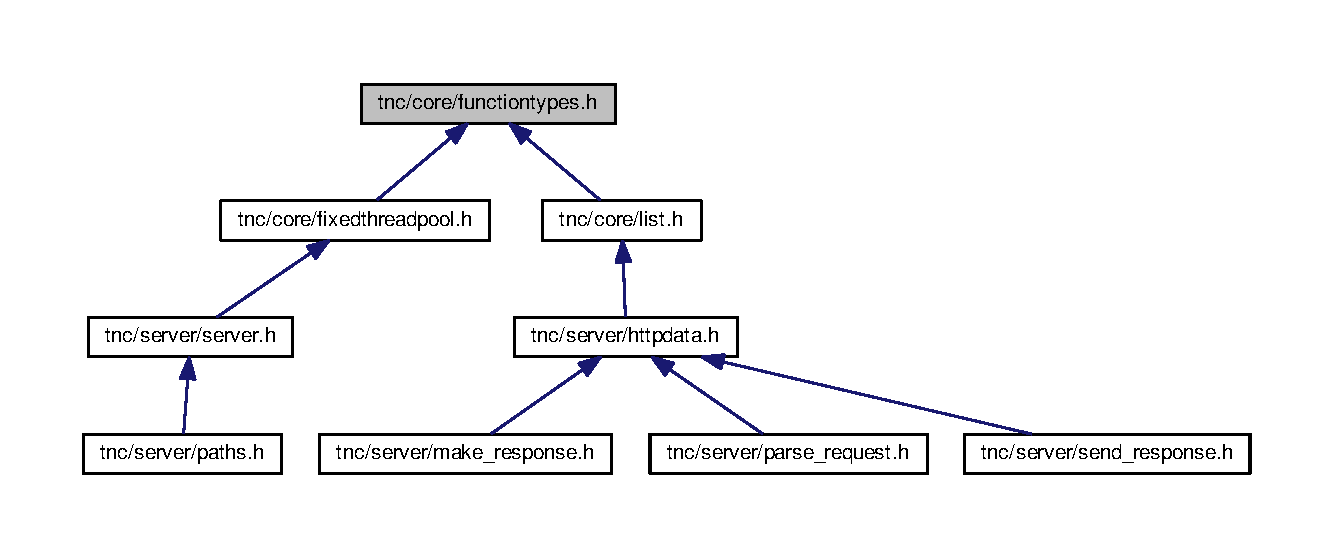
\includegraphics[width=350pt]{functiontypes_8h__dep__incl}
\end{center}
\end{figure}
\subsection*{Ridefinizioni di tipo (typedef)}
\begin{DoxyCompactItemize}
\item 
typedef void($\ast$ \hyperlink{functiontypes_8h_a78b4c663dde4687b8cddd1ca6031cadb}{T\+N\+C\+Consumer}) (void $\ast$)
\begin{DoxyCompactList}\small\item\em Alias a puntatore di funzione void(void$\ast$). \end{DoxyCompactList}\item 
typedef void $\ast$($\ast$ \hyperlink{functiontypes_8h_ab55be5b67db12c27273a3598b1be3d8a}{T\+N\+C\+Function}) (void $\ast$)
\begin{DoxyCompactList}\small\item\em Alias a puntatore di funzione void$\ast$(void$\ast$). \end{DoxyCompactList}\end{DoxyCompactItemize}


\subsection{Descrizione dettagliata}
Contiene alias a tipo di puntatore a funzione. 



\subsection{Documentazione delle ridefinizioni di tipo (typedef)}
\hypertarget{functiontypes_8h_a78b4c663dde4687b8cddd1ca6031cadb}{}\index{functiontypes.\+h@{functiontypes.\+h}!T\+N\+C\+Consumer@{T\+N\+C\+Consumer}}
\index{T\+N\+C\+Consumer@{T\+N\+C\+Consumer}!functiontypes.\+h@{functiontypes.\+h}}
\subsubsection[{T\+N\+C\+Consumer}]{\setlength{\rightskip}{0pt plus 5cm}typedef void($\ast$ T\+N\+C\+Consumer) (void $\ast$)}\label{functiontypes_8h_a78b4c663dde4687b8cddd1ca6031cadb}


Alias a puntatore di funzione void(void$\ast$). 

\hypertarget{functiontypes_8h_ab55be5b67db12c27273a3598b1be3d8a}{}\index{functiontypes.\+h@{functiontypes.\+h}!T\+N\+C\+Function@{T\+N\+C\+Function}}
\index{T\+N\+C\+Function@{T\+N\+C\+Function}!functiontypes.\+h@{functiontypes.\+h}}
\subsubsection[{T\+N\+C\+Function}]{\setlength{\rightskip}{0pt plus 5cm}typedef void$\ast$($\ast$ T\+N\+C\+Function) (void $\ast$)}\label{functiontypes_8h_ab55be5b67db12c27273a3598b1be3d8a}


Alias a puntatore di funzione void$\ast$(void$\ast$). 


\hypertarget{list_8h}{}\section{Riferimenti per il file tnc/core/list.h}
\label{list_8h}\index{tnc/core/list.\+h@{tnc/core/list.\+h}}


Contiene l\textquotesingle{}interfaccia per le liste doppiamente concatenate.  


{\ttfamily \#include \char`\"{}functiontypes.\+h\char`\"{}}\\*
Grafo delle dipendenze di inclusione per list.\+h\+:\nopagebreak
\begin{figure}[H]
\begin{center}
\leavevmode
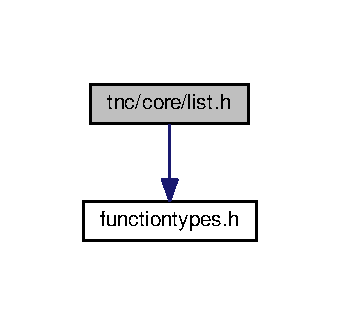
\includegraphics[width=163pt]{list_8h__incl}
\end{center}
\end{figure}
Questo grafo mostra quali altri file includono direttamente o indirettamente questo file\+:\nopagebreak
\begin{figure}[H]
\begin{center}
\leavevmode
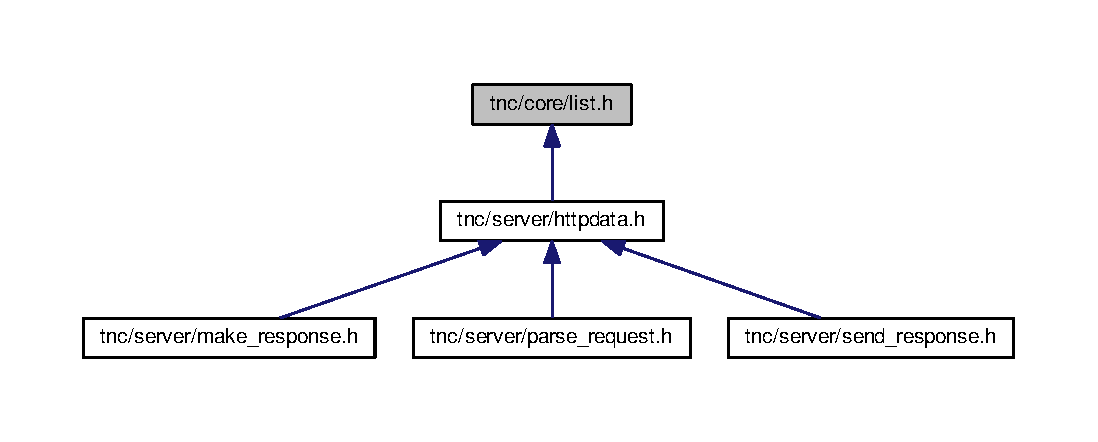
\includegraphics[width=350pt]{list_8h__dep__incl}
\end{center}
\end{figure}
\subsection*{Funzioni}
\begin{DoxyCompactItemize}
\item 
T\+N\+C\+List \hyperlink{list_8h_a348c5bc63c91ace3343370373f4328b0}{T\+N\+C\+List\+\_\+new} ()
\begin{DoxyCompactList}\small\item\em Inizializza una lista. \end{DoxyCompactList}\item 
T\+N\+C\+List\+Node \hyperlink{list_8h_ac5e4d9ffa5af8ceb91f384b562a9d6bf}{T\+N\+C\+List\+\_\+first} (T\+N\+C\+List list)
\begin{DoxyCompactList}\small\item\em Restituisce il primo nodo di una lista. \end{DoxyCompactList}\item 
T\+N\+C\+List\+Node \hyperlink{list_8h_ad81a2d6c8ef1fa5390fd0b1c59f49728}{T\+N\+C\+List\+\_\+last} (T\+N\+C\+List list)
\begin{DoxyCompactList}\small\item\em Restituisce l\textquotesingle{}ultimo nodo di una lista. \end{DoxyCompactList}\item 
T\+N\+C\+List\+Node \hyperlink{list_8h_ae7534b594aa3353a3f27313442ffd0ba}{T\+N\+C\+List\+\_\+next} (T\+N\+C\+List\+Node current)
\begin{DoxyCompactList}\small\item\em Restituisce il nodo successivo in una lista rispetto a un nodo passato come parametro. \end{DoxyCompactList}\item 
T\+N\+C\+List\+Node \hyperlink{list_8h_a1b7a902b8a8a5b78e91b07ff56591e24}{T\+N\+C\+List\+\_\+previous} (T\+N\+C\+List\+Node current)
\begin{DoxyCompactList}\small\item\em Restituisce il nodo precedente in una lista rispetto a un nodo passato come parametro. \end{DoxyCompactList}\item 
int \hyperlink{list_8h_af90bc4481504329ec71a3f06916e56ca}{T\+N\+C\+List\+\_\+push\+\_\+front} (T\+N\+C\+List restrict self, void $\ast$restrict val)
\begin{DoxyCompactList}\small\item\em Inserisce un nuovo nodo come primo elemento della lista. \end{DoxyCompactList}\item 
int \hyperlink{list_8h_aa16018ceeb34a5efff57b582c7387d89}{T\+N\+C\+List\+\_\+push\+\_\+back} (T\+N\+C\+List restrict self, void $\ast$restrict val)
\begin{DoxyCompactList}\small\item\em Inserisce un nuovo nodo come ultimo elemento della lista. \end{DoxyCompactList}\item 
int \hyperlink{list_8h_a5642341347cf8ceb18c96097478da28f}{T\+N\+C\+List\+\_\+insert\+\_\+before} (T\+N\+C\+List\+Node restrict ref, void $\ast$restrict val)
\begin{DoxyCompactList}\small\item\em Inserisce un elemento prima del nodo passato come parametro. \end{DoxyCompactList}\item 
int \hyperlink{list_8h_a1e8317df833ce5fe88a94cda4e4310b2}{T\+N\+C\+List\+\_\+insert\+\_\+after} (T\+N\+C\+List\+Node restrict ref, void $\ast$restrict val)
\begin{DoxyCompactList}\small\item\em Inserisce un elemento dopo il nodo passato come parametro. \end{DoxyCompactList}\item 
void $\ast$ \hyperlink{list_8h_a4e2ce6ee419787d2b4a1a36a1ec38341}{T\+N\+C\+List\+\_\+pop\+\_\+front} (T\+N\+C\+List self)
\begin{DoxyCompactList}\small\item\em Toglie il primo elemento dalla lista, e lo restituisce. \end{DoxyCompactList}\item 
void $\ast$ \hyperlink{list_8h_ae66d30798518d1a83ea84c45ad90b843}{T\+N\+C\+List\+\_\+pop\+\_\+back} (T\+N\+C\+List self)
\begin{DoxyCompactList}\small\item\em Toglie l\textquotesingle{}ultimo elemento dalla lista, e lo restituisce. \end{DoxyCompactList}\item 
void $\ast$ \hyperlink{list_8h_aefa18bb9ec9638f5b25d0c596460ced2}{T\+N\+C\+List\+\_\+remove} (T\+N\+C\+List\+Node node)
\begin{DoxyCompactList}\small\item\em Rimuove un elemento da una lista. \end{DoxyCompactList}\item 
const void $\ast$ \hyperlink{list_8h_aab379437b73d4b40caff1d7e8b1cd216}{T\+N\+C\+List\+\_\+getvalue} (T\+N\+C\+List\+Node node)
\begin{DoxyCompactList}\small\item\em Dato un nodo, restituisce un puntatore costante al suo valore. \end{DoxyCompactList}\item 
void \hyperlink{list_8h_a366497def8fb6151756bcec9424bce95}{T\+N\+C\+List\+\_\+destroy} (T\+N\+C\+List self)
\begin{DoxyCompactList}\small\item\em Cancella (dealloca) una lista. \end{DoxyCompactList}\item 
void \hyperlink{list_8h_aae5c3c2385ae5018a3181151140d6841}{T\+N\+C\+List\+\_\+destroy\+\_\+and\+\_\+free} (T\+N\+C\+List self, \hyperlink{functiontypes_8h_a78b4c663dde4687b8cddd1ca6031cadb}{T\+N\+C\+Consumer} freefn)
\begin{DoxyCompactList}\small\item\em Cancella una lista e chiama una funzione su tutti i suoi elementi. \end{DoxyCompactList}\item 
void \hyperlink{list_8h_ac16e5d1d334f64f619605aab7834e0f3}{T\+N\+C\+List\+\_\+chain} (T\+N\+C\+List restrict list, T\+N\+C\+List restrict to\+\_\+chain)
\begin{DoxyCompactList}\small\item\em Concatena due liste. \end{DoxyCompactList}\item 
\hypertarget{list_8h_a841ef92f69f013a3e28a37a0cacba52f}{}int \hyperlink{list_8h_a841ef92f69f013a3e28a37a0cacba52f}{T\+N\+C\+List\+\_\+empty} (T\+N\+C\+List self)\label{list_8h_a841ef92f69f013a3e28a37a0cacba52f}

\begin{DoxyCompactList}\small\item\em Restituisce un valore diverso da zero se la lista è vuota, altrimenti 0. \end{DoxyCompactList}\item 
\hypertarget{list_8h_a062188a59982a6022f5928092b4111c1}{}size\+\_\+t \hyperlink{list_8h_a062188a59982a6022f5928092b4111c1}{T\+N\+C\+List\+\_\+length} (T\+N\+C\+List self)\label{list_8h_a062188a59982a6022f5928092b4111c1}

\begin{DoxyCompactList}\small\item\em Restituisce il numero di elementi in una lista. \end{DoxyCompactList}\end{DoxyCompactItemize}


\subsection{Descrizione dettagliata}
Contiene l\textquotesingle{}interfaccia per le liste doppiamente concatenate. 



\subsection{Documentazione delle funzioni}
\hypertarget{list_8h_ac16e5d1d334f64f619605aab7834e0f3}{}\index{list.\+h@{list.\+h}!T\+N\+C\+List\+\_\+chain@{T\+N\+C\+List\+\_\+chain}}
\index{T\+N\+C\+List\+\_\+chain@{T\+N\+C\+List\+\_\+chain}!list.\+h@{list.\+h}}
\subsubsection[{T\+N\+C\+List\+\_\+chain}]{\setlength{\rightskip}{0pt plus 5cm}void T\+N\+C\+List\+\_\+chain (
\begin{DoxyParamCaption}
\item[{T\+N\+C\+List restrict}]{list, }
\item[{T\+N\+C\+List restrict}]{to\+\_\+chain}
\end{DoxyParamCaption}
)}\label{list_8h_ac16e5d1d334f64f619605aab7834e0f3}


Concatena due liste. 


\begin{DoxyParams}{Parametri}
{\em list} & La lista con i primi elementi. Alla conclusione della funzione, questa lista conterrà le due liste concatenate. Questo parametro non deve essere N\+U\+L\+L.\\
\hline
{\em to\+\_\+chain} & La seconda lista da concatenare. Questa lista viene distrutta al termine della funzione. Questo parametro non deve essere N\+U\+L\+L. \\
\hline
\end{DoxyParams}
\hypertarget{list_8h_a366497def8fb6151756bcec9424bce95}{}\index{list.\+h@{list.\+h}!T\+N\+C\+List\+\_\+destroy@{T\+N\+C\+List\+\_\+destroy}}
\index{T\+N\+C\+List\+\_\+destroy@{T\+N\+C\+List\+\_\+destroy}!list.\+h@{list.\+h}}
\subsubsection[{T\+N\+C\+List\+\_\+destroy}]{\setlength{\rightskip}{0pt plus 5cm}void T\+N\+C\+List\+\_\+destroy (
\begin{DoxyParamCaption}
\item[{T\+N\+C\+List}]{self}
\end{DoxyParamCaption}
)}\label{list_8h_a366497def8fb6151756bcec9424bce95}


Cancella (dealloca) una lista. 


\begin{DoxyParams}{Parametri}
{\em self} & La lista da cancellare \\
\hline
\end{DoxyParams}
\hypertarget{list_8h_aae5c3c2385ae5018a3181151140d6841}{}\index{list.\+h@{list.\+h}!T\+N\+C\+List\+\_\+destroy\+\_\+and\+\_\+free@{T\+N\+C\+List\+\_\+destroy\+\_\+and\+\_\+free}}
\index{T\+N\+C\+List\+\_\+destroy\+\_\+and\+\_\+free@{T\+N\+C\+List\+\_\+destroy\+\_\+and\+\_\+free}!list.\+h@{list.\+h}}
\subsubsection[{T\+N\+C\+List\+\_\+destroy\+\_\+and\+\_\+free}]{\setlength{\rightskip}{0pt plus 5cm}void T\+N\+C\+List\+\_\+destroy\+\_\+and\+\_\+free (
\begin{DoxyParamCaption}
\item[{T\+N\+C\+List}]{self, }
\item[{{\bf T\+N\+C\+Consumer}}]{freefn}
\end{DoxyParamCaption}
)}\label{list_8h_aae5c3c2385ae5018a3181151140d6841}


Cancella una lista e chiama una funzione su tutti i suoi elementi. 


\begin{DoxyParams}{Parametri}
{\em self} & La lista da cancellare\\
\hline
{\em freefn} & Un puntatore a una funzione di deallocazione da chiamare per ogni elemento nella lista. Se N\+U\+L\+L, nessuna funzione verrà chiamata e gli elementi non verranno deallocati. \\
\hline
\end{DoxyParams}
\hypertarget{list_8h_ac5e4d9ffa5af8ceb91f384b562a9d6bf}{}\index{list.\+h@{list.\+h}!T\+N\+C\+List\+\_\+first@{T\+N\+C\+List\+\_\+first}}
\index{T\+N\+C\+List\+\_\+first@{T\+N\+C\+List\+\_\+first}!list.\+h@{list.\+h}}
\subsubsection[{T\+N\+C\+List\+\_\+first}]{\setlength{\rightskip}{0pt plus 5cm}T\+N\+C\+List\+Node T\+N\+C\+List\+\_\+first (
\begin{DoxyParamCaption}
\item[{T\+N\+C\+List}]{list}
\end{DoxyParamCaption}
)}\label{list_8h_ac5e4d9ffa5af8ceb91f384b562a9d6bf}


Restituisce il primo nodo di una lista. 


\begin{DoxyParams}{Parametri}
{\em list} & La lista su cui si vuole operare. Il comportamento della funzione non è definito se questo parametro è N\+U\+L\+L.\\
\hline
\end{DoxyParams}
\begin{DoxyReturn}{Restituisce}
Un T\+N\+C\+List\+Node corrispondente al primo nodo della lista, N\+U\+L\+L se la lista è vuota. 
\end{DoxyReturn}
\hypertarget{list_8h_aab379437b73d4b40caff1d7e8b1cd216}{}\index{list.\+h@{list.\+h}!T\+N\+C\+List\+\_\+getvalue@{T\+N\+C\+List\+\_\+getvalue}}
\index{T\+N\+C\+List\+\_\+getvalue@{T\+N\+C\+List\+\_\+getvalue}!list.\+h@{list.\+h}}
\subsubsection[{T\+N\+C\+List\+\_\+getvalue}]{\setlength{\rightskip}{0pt plus 5cm}const void$\ast$ T\+N\+C\+List\+\_\+getvalue (
\begin{DoxyParamCaption}
\item[{T\+N\+C\+List\+Node}]{node}
\end{DoxyParamCaption}
)}\label{list_8h_aab379437b73d4b40caff1d7e8b1cd216}


Dato un nodo, restituisce un puntatore costante al suo valore. 


\begin{DoxyParams}{Parametri}
{\em node} & Il nodo di cui si richiede il valore. Il comportamento della funzione è indefinito se questo parametro è N\+U\+L\+L.\\
\hline
\end{DoxyParams}
\begin{DoxyReturn}{Restituisce}
Il valore corrispondente al nodo 
\end{DoxyReturn}
\hypertarget{list_8h_a1e8317df833ce5fe88a94cda4e4310b2}{}\index{list.\+h@{list.\+h}!T\+N\+C\+List\+\_\+insert\+\_\+after@{T\+N\+C\+List\+\_\+insert\+\_\+after}}
\index{T\+N\+C\+List\+\_\+insert\+\_\+after@{T\+N\+C\+List\+\_\+insert\+\_\+after}!list.\+h@{list.\+h}}
\subsubsection[{T\+N\+C\+List\+\_\+insert\+\_\+after}]{\setlength{\rightskip}{0pt plus 5cm}int T\+N\+C\+List\+\_\+insert\+\_\+after (
\begin{DoxyParamCaption}
\item[{T\+N\+C\+List\+Node restrict}]{ref, }
\item[{void $\ast$restrict}]{val}
\end{DoxyParamCaption}
)}\label{list_8h_a1e8317df833ce5fe88a94cda4e4310b2}


Inserisce un elemento dopo il nodo passato come parametro. 


\begin{DoxyParams}{Parametri}
{\em ref} & Il nodo di riferimento. Il comportamento della funzione non è definito se questo parametro è N\+U\+L\+L.\\
\hline
{\em val} & Elemento da inserire nella lista\\
\hline
\end{DoxyParams}
\begin{DoxyReturn}{Restituisce}
0 se l\textquotesingle{}operazione va a buon fine, altrimenti uno dei seguenti codici di errore\+: -\/ T\+N\+C\+Error\+\_\+failed\+\_\+alloc se non è stato possibile allocare memoria per eseguire l\textquotesingle{}operazione. 
\end{DoxyReturn}
\hypertarget{list_8h_a5642341347cf8ceb18c96097478da28f}{}\index{list.\+h@{list.\+h}!T\+N\+C\+List\+\_\+insert\+\_\+before@{T\+N\+C\+List\+\_\+insert\+\_\+before}}
\index{T\+N\+C\+List\+\_\+insert\+\_\+before@{T\+N\+C\+List\+\_\+insert\+\_\+before}!list.\+h@{list.\+h}}
\subsubsection[{T\+N\+C\+List\+\_\+insert\+\_\+before}]{\setlength{\rightskip}{0pt plus 5cm}int T\+N\+C\+List\+\_\+insert\+\_\+before (
\begin{DoxyParamCaption}
\item[{T\+N\+C\+List\+Node restrict}]{ref, }
\item[{void $\ast$restrict}]{val}
\end{DoxyParamCaption}
)}\label{list_8h_a5642341347cf8ceb18c96097478da28f}


Inserisce un elemento prima del nodo passato come parametro. 


\begin{DoxyParams}{Parametri}
{\em ref} & Il nodo di riferimento. Il comportamento della funzione non è definito se questo parametro è N\+U\+L\+L.\\
\hline
{\em val} & Elemento da inserire nella lista\\
\hline
\end{DoxyParams}
\begin{DoxyReturn}{Restituisce}
0 se l\textquotesingle{}operazione va a buon fine, altrimenti uno dei seguenti codici di errore\+: -\/ T\+N\+C\+Error\+\_\+failed\+\_\+alloc se non è stato possibile allocare memoria per eseguire l\textquotesingle{}operazione. 
\end{DoxyReturn}
\hypertarget{list_8h_ad81a2d6c8ef1fa5390fd0b1c59f49728}{}\index{list.\+h@{list.\+h}!T\+N\+C\+List\+\_\+last@{T\+N\+C\+List\+\_\+last}}
\index{T\+N\+C\+List\+\_\+last@{T\+N\+C\+List\+\_\+last}!list.\+h@{list.\+h}}
\subsubsection[{T\+N\+C\+List\+\_\+last}]{\setlength{\rightskip}{0pt plus 5cm}T\+N\+C\+List\+Node T\+N\+C\+List\+\_\+last (
\begin{DoxyParamCaption}
\item[{T\+N\+C\+List}]{list}
\end{DoxyParamCaption}
)}\label{list_8h_ad81a2d6c8ef1fa5390fd0b1c59f49728}


Restituisce l\textquotesingle{}ultimo nodo di una lista. 


\begin{DoxyParams}{Parametri}
{\em list} & La lista su cui si vuole operare. Il\\
\hline
\end{DoxyParams}
\begin{DoxyReturn}{Restituisce}
Un T\+N\+C\+List\+Node corrispondente all\textquotesingle{}ultimo nodo della lista, N\+U\+L\+L se la lista è vuota.
\end{DoxyReturn}
\begin{DoxySeeAlso}{Si veda anche}
T\+N\+C\+List\+Node 
\end{DoxySeeAlso}
\hypertarget{list_8h_a348c5bc63c91ace3343370373f4328b0}{}\index{list.\+h@{list.\+h}!T\+N\+C\+List\+\_\+new@{T\+N\+C\+List\+\_\+new}}
\index{T\+N\+C\+List\+\_\+new@{T\+N\+C\+List\+\_\+new}!list.\+h@{list.\+h}}
\subsubsection[{T\+N\+C\+List\+\_\+new}]{\setlength{\rightskip}{0pt plus 5cm}T\+N\+C\+List T\+N\+C\+List\+\_\+new (
\begin{DoxyParamCaption}
{}
\end{DoxyParamCaption}
)}\label{list_8h_a348c5bc63c91ace3343370373f4328b0}


Inizializza una lista. 

\begin{DoxyReturn}{Restituisce}
Un puntatore a una lista inizializzata se l\textquotesingle{}allocazione va a buon fine, N\+U\+L\+L altrimenti. 
\end{DoxyReturn}
\hypertarget{list_8h_ae7534b594aa3353a3f27313442ffd0ba}{}\index{list.\+h@{list.\+h}!T\+N\+C\+List\+\_\+next@{T\+N\+C\+List\+\_\+next}}
\index{T\+N\+C\+List\+\_\+next@{T\+N\+C\+List\+\_\+next}!list.\+h@{list.\+h}}
\subsubsection[{T\+N\+C\+List\+\_\+next}]{\setlength{\rightskip}{0pt plus 5cm}T\+N\+C\+List\+Node T\+N\+C\+List\+\_\+next (
\begin{DoxyParamCaption}
\item[{T\+N\+C\+List\+Node}]{current}
\end{DoxyParamCaption}
)}\label{list_8h_ae7534b594aa3353a3f27313442ffd0ba}


Restituisce il nodo successivo in una lista rispetto a un nodo passato come parametro. 


\begin{DoxyParams}{Parametri}
{\em current} & Il nodo di cui si vuole conoscere l\textquotesingle{}elemento successivo. Il parametro deve essere un nodo valido di una lista (non deve essere N\+U\+L\+L e non deve essere un nodo che è stato rimosso).\\
\hline
\end{DoxyParams}
\begin{DoxyReturn}{Restituisce}
Il nodo della lista successivo a quello passato come parametro. N\+U\+L\+L se current è l\textquotesingle{}ultimo nodo della lista.
\end{DoxyReturn}
\begin{DoxySeeAlso}{Si veda anche}
T\+N\+C\+List\+Node 
\end{DoxySeeAlso}
\hypertarget{list_8h_ae66d30798518d1a83ea84c45ad90b843}{}\index{list.\+h@{list.\+h}!T\+N\+C\+List\+\_\+pop\+\_\+back@{T\+N\+C\+List\+\_\+pop\+\_\+back}}
\index{T\+N\+C\+List\+\_\+pop\+\_\+back@{T\+N\+C\+List\+\_\+pop\+\_\+back}!list.\+h@{list.\+h}}
\subsubsection[{T\+N\+C\+List\+\_\+pop\+\_\+back}]{\setlength{\rightskip}{0pt plus 5cm}void$\ast$ T\+N\+C\+List\+\_\+pop\+\_\+back (
\begin{DoxyParamCaption}
\item[{T\+N\+C\+List}]{self}
\end{DoxyParamCaption}
)}\label{list_8h_ae66d30798518d1a83ea84c45ad90b843}


Toglie l\textquotesingle{}ultimo elemento dalla lista, e lo restituisce. 


\begin{DoxyParams}{Parametri}
{\em self} & La lista su cui si vuole operare. Il comportamento della funzione non è definito se questo parametro è N\+U\+L\+L o se la lista a cui si riferisce è vuota. \\
\hline
\end{DoxyParams}
\hypertarget{list_8h_a4e2ce6ee419787d2b4a1a36a1ec38341}{}\index{list.\+h@{list.\+h}!T\+N\+C\+List\+\_\+pop\+\_\+front@{T\+N\+C\+List\+\_\+pop\+\_\+front}}
\index{T\+N\+C\+List\+\_\+pop\+\_\+front@{T\+N\+C\+List\+\_\+pop\+\_\+front}!list.\+h@{list.\+h}}
\subsubsection[{T\+N\+C\+List\+\_\+pop\+\_\+front}]{\setlength{\rightskip}{0pt plus 5cm}void$\ast$ T\+N\+C\+List\+\_\+pop\+\_\+front (
\begin{DoxyParamCaption}
\item[{T\+N\+C\+List}]{self}
\end{DoxyParamCaption}
)}\label{list_8h_a4e2ce6ee419787d2b4a1a36a1ec38341}


Toglie il primo elemento dalla lista, e lo restituisce. 


\begin{DoxyParams}{Parametri}
{\em self} & La lista su cui si vuole operare Il comportamento della funzione non è definito se questo parametro è N\+U\+L\+L o se la lista a cui si riferisce è vuota.\\
\hline
\end{DoxyParams}
\begin{DoxyReturn}{Restituisce}
0 se l\textquotesingle{}operazione va a buon fine, altrimenti uno dei seguenti codici di errore\+: -\/ T\+N\+C\+Error\+\_\+failed\+\_\+alloc se non è stato possibile allocare memoria per eseguire l\textquotesingle{}operazione. 
\end{DoxyReturn}
\hypertarget{list_8h_a1b7a902b8a8a5b78e91b07ff56591e24}{}\index{list.\+h@{list.\+h}!T\+N\+C\+List\+\_\+previous@{T\+N\+C\+List\+\_\+previous}}
\index{T\+N\+C\+List\+\_\+previous@{T\+N\+C\+List\+\_\+previous}!list.\+h@{list.\+h}}
\subsubsection[{T\+N\+C\+List\+\_\+previous}]{\setlength{\rightskip}{0pt plus 5cm}T\+N\+C\+List\+Node T\+N\+C\+List\+\_\+previous (
\begin{DoxyParamCaption}
\item[{T\+N\+C\+List\+Node}]{current}
\end{DoxyParamCaption}
)}\label{list_8h_a1b7a902b8a8a5b78e91b07ff56591e24}


Restituisce il nodo precedente in una lista rispetto a un nodo passato come parametro. 


\begin{DoxyParams}{Parametri}
{\em current} & Il nodo di cui si vuole conoscere l\textquotesingle{}elemento precedente. Il parametro deve essere un nodo valido di una lista (non deve essere N\+U\+L\+L e non deve essere un nodo che è stato rimosso).\\
\hline
\end{DoxyParams}
\begin{DoxyReturn}{Restituisce}
Il nodo della lista successivo a quello passato come parametro. N\+U\+L\+L se current è il primo nodo della lista.
\end{DoxyReturn}
\begin{DoxySeeAlso}{Si veda anche}
T\+N\+C\+List\+Node 
\end{DoxySeeAlso}
\hypertarget{list_8h_aa16018ceeb34a5efff57b582c7387d89}{}\index{list.\+h@{list.\+h}!T\+N\+C\+List\+\_\+push\+\_\+back@{T\+N\+C\+List\+\_\+push\+\_\+back}}
\index{T\+N\+C\+List\+\_\+push\+\_\+back@{T\+N\+C\+List\+\_\+push\+\_\+back}!list.\+h@{list.\+h}}
\subsubsection[{T\+N\+C\+List\+\_\+push\+\_\+back}]{\setlength{\rightskip}{0pt plus 5cm}int T\+N\+C\+List\+\_\+push\+\_\+back (
\begin{DoxyParamCaption}
\item[{T\+N\+C\+List restrict}]{self, }
\item[{void $\ast$restrict}]{val}
\end{DoxyParamCaption}
)}\label{list_8h_aa16018ceeb34a5efff57b582c7387d89}


Inserisce un nuovo nodo come ultimo elemento della lista. 


\begin{DoxyParams}{Parametri}
{\em self} & La lista su cui si vuole operare. Il comportamento della funzione non è definito se questo parametro è N\+U\+L\+L.\\
\hline
{\em val} & Elemento da inserire nella lista.\\
\hline
\end{DoxyParams}
\begin{DoxyReturn}{Restituisce}
0 se l\textquotesingle{}operazione va a buon fine, altrimenti uno dei seguenti codici di errore\+: -\/ T\+N\+C\+Error\+\_\+failed\+\_\+alloc se non è stato possibile allocare memoria per eseguire l\textquotesingle{}operazione. 
\end{DoxyReturn}
\hypertarget{list_8h_af90bc4481504329ec71a3f06916e56ca}{}\index{list.\+h@{list.\+h}!T\+N\+C\+List\+\_\+push\+\_\+front@{T\+N\+C\+List\+\_\+push\+\_\+front}}
\index{T\+N\+C\+List\+\_\+push\+\_\+front@{T\+N\+C\+List\+\_\+push\+\_\+front}!list.\+h@{list.\+h}}
\subsubsection[{T\+N\+C\+List\+\_\+push\+\_\+front}]{\setlength{\rightskip}{0pt plus 5cm}int T\+N\+C\+List\+\_\+push\+\_\+front (
\begin{DoxyParamCaption}
\item[{T\+N\+C\+List restrict}]{self, }
\item[{void $\ast$restrict}]{val}
\end{DoxyParamCaption}
)}\label{list_8h_af90bc4481504329ec71a3f06916e56ca}


Inserisce un nuovo nodo come primo elemento della lista. 


\begin{DoxyParams}{Parametri}
{\em self} & La lista su cui si vuole operare. Il comportamento della funzione non è definito se questo parametro è N\+U\+L\+L.\\
\hline
{\em val} & Il nuovo elemento da inserire nella lista.\\
\hline
\end{DoxyParams}
\begin{DoxyReturn}{Restituisce}
0 se l\textquotesingle{}operazione va a buon fine, altrimenti uno dei seguenti codici di errore\+: -\/ T\+N\+C\+Error\+\_\+failed\+\_\+alloc se non è stato possibile allocare memoria per eseguire l\textquotesingle{}operazione.
\end{DoxyReturn}
\begin{DoxySeeAlso}{Si veda anche}
T\+N\+C\+List\+Node 

error.\+h 
\end{DoxySeeAlso}
\hypertarget{list_8h_aefa18bb9ec9638f5b25d0c596460ced2}{}\index{list.\+h@{list.\+h}!T\+N\+C\+List\+\_\+remove@{T\+N\+C\+List\+\_\+remove}}
\index{T\+N\+C\+List\+\_\+remove@{T\+N\+C\+List\+\_\+remove}!list.\+h@{list.\+h}}
\subsubsection[{T\+N\+C\+List\+\_\+remove}]{\setlength{\rightskip}{0pt plus 5cm}void$\ast$ T\+N\+C\+List\+\_\+remove (
\begin{DoxyParamCaption}
\item[{T\+N\+C\+List\+Node}]{node}
\end{DoxyParamCaption}
)}\label{list_8h_aefa18bb9ec9638f5b25d0c596460ced2}


Rimuove un elemento da una lista. 


\begin{DoxyParams}{Parametri}
{\em node} & Il nodo corrispondente all\textquotesingle{}elemento da togliere. Se N\+U\+L\+L, il comportamento della funzione non è definito.\\
\hline
{\em freefn} & Una funzione da chiamare per dellocare l\textquotesingle{}elemento. Se N\+U\+L\+L, non viene chiamata nessuna funzione sull\textquotesingle{}elemento e questo non viene deallocato. \\
\hline
\end{DoxyParams}

\hypertarget{httpdata_8h}{}\section{Riferimenti per il file tnc/server/httpdata.h}
\label{httpdata_8h}\index{tnc/server/httpdata.\+h@{tnc/server/httpdata.\+h}}


Contiene strutture dati utili al salvataggio dei dati delle richieste e delle risposte H\+T\+T\+P.  


{\ttfamily \#include $<$stdbool.\+h$>$}\\*
{\ttfamily \#include $<$stdio.\+h$>$}\\*
{\ttfamily \#include $<$stdint.\+h$>$}\\*
{\ttfamily \#include $<$time.\+h$>$}\\*
{\ttfamily \#include \char`\"{}httpheaders.\+h\char`\"{}}\\*
{\ttfamily \#include \char`\"{}tnc/core/list.\+h\char`\"{}}\\*
Grafo delle dipendenze di inclusione per httpdata.\+h\+:\nopagebreak
\begin{figure}[H]
\begin{center}
\leavevmode
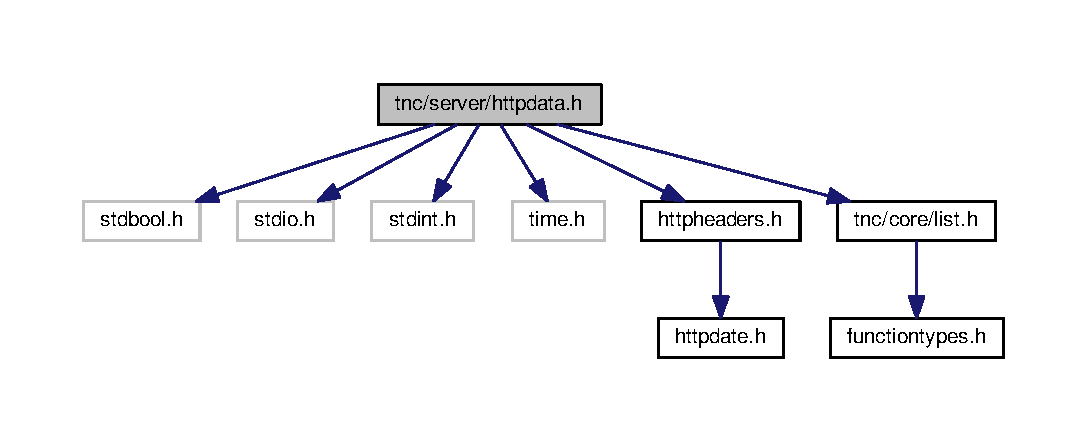
\includegraphics[width=350pt]{httpdata_8h__incl}
\end{center}
\end{figure}
Questo grafo mostra quali altri file includono direttamente o indirettamente questo file\+:\nopagebreak
\begin{figure}[H]
\begin{center}
\leavevmode
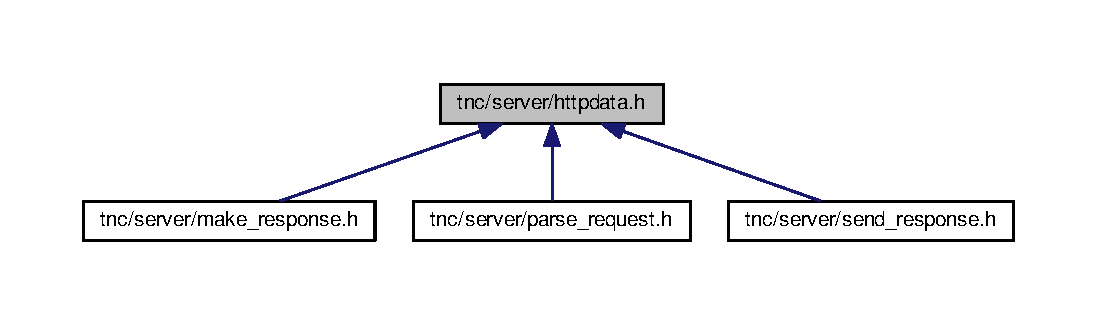
\includegraphics[width=350pt]{httpdata_8h__dep__incl}
\end{center}
\end{figure}
\subsection*{Strutture dati}
\begin{DoxyCompactItemize}
\item 
struct \hyperlink{structHTTPRequestData}{H\+T\+T\+P\+Request\+Data}
\begin{DoxyCompactList}\small\item\em Contiene informazioni su di una richiesta H\+T\+T\+P. \end{DoxyCompactList}\item 
struct \hyperlink{structHTTPRequestHeader}{H\+T\+T\+P\+Request\+Header}
\begin{DoxyCompactList}\small\item\em Rappresenta un header di richiesta H\+T\+T\+P. \end{DoxyCompactList}\item 
struct \hyperlink{structHTTPResponseData}{H\+T\+T\+P\+Response\+Data}
\end{DoxyCompactItemize}
\subsection*{Tipi enumerati (enum)}
\begin{DoxyCompactItemize}
\item 
enum \hyperlink{httpdata_8h_a159dd434f3cab184e5fab8365ed494ec}{H\+T\+T\+P\+Request\+Data\+\_\+flags} \{ \hyperlink{httpdata_8h_a159dd434f3cab184e5fab8365ed494eca38f1b00cb61c162432d579553dfc4f98}{H\+T\+T\+P\+Request\+Data\+\_\+flags\+\_\+stop\+\_\+parsing} = 1 $<$$<$ 0, 
\hyperlink{httpdata_8h_a159dd434f3cab184e5fab8365ed494eca9f170ca51d662124859bfd11df8f24e4}{H\+T\+T\+P\+Request\+Data\+\_\+flags\+\_\+keep\+\_\+alive} = 1 $<$$<$ 1, 
\hyperlink{httpdata_8h_a159dd434f3cab184e5fab8365ed494ecac2cce33be3baf44d3f60e19084ae311f}{H\+T\+T\+P\+Request\+Data\+\_\+flags\+\_\+dont\+\_\+send\+\_\+payload} = 1 $<$$<$ 2, 
\hyperlink{httpdata_8h_a159dd434f3cab184e5fab8365ed494eca0a19f89674a79292d364b01350b56657}{H\+T\+T\+P\+Request\+Data\+\_\+flags\+\_\+get\+\_\+error\+\_\+page} = 1 $<$$<$ 3
 \}
\begin{DoxyCompactList}\small\item\em I valori di questa enumerazione vengono usati per creare una bitmask che rappresenta informazioni e istruzioni di operazione per la richiesta H\+T\+T\+P a cui si riferiscono. \end{DoxyCompactList}\end{DoxyCompactItemize}
\subsection*{Funzioni}
\begin{DoxyCompactItemize}
\item 
\hypertarget{httpdata_8h_aae80dcf2f216067f2defd6ba687a0c18}{}void {\bfseries H\+T\+T\+P\+Request\+Data\+\_\+init} (\hyperlink{structHTTPRequestData}{H\+T\+T\+P\+Request\+Data} $\ast$data)\label{httpdata_8h_aae80dcf2f216067f2defd6ba687a0c18}

\item 
\hypertarget{httpdata_8h_a4ee0b3da0116b245db6987d1cfd695f7}{}\hyperlink{structHTTPRequestData}{H\+T\+T\+P\+Request\+Data} $\ast$ {\bfseries H\+T\+T\+P\+Request\+Data\+\_\+new} ()\label{httpdata_8h_a4ee0b3da0116b245db6987d1cfd695f7}

\item 
\hypertarget{httpdata_8h_a8ded1ce540f51d34b8176a5208eca79e}{}void {\bfseries H\+T\+T\+P\+Request\+Data\+\_\+destroy} (\hyperlink{structHTTPRequestData}{H\+T\+T\+P\+Request\+Data} $\ast$data)\label{httpdata_8h_a8ded1ce540f51d34b8176a5208eca79e}

\item 
\hypertarget{httpdata_8h_a04b45ca7a5a8659fa67f69dba491f59b}{}void {\bfseries H\+T\+T\+P\+Request\+Data\+\_\+destroy\+\_\+members} (\hyperlink{structHTTPRequestData}{H\+T\+T\+P\+Request\+Data} $\ast$data)\label{httpdata_8h_a04b45ca7a5a8659fa67f69dba491f59b}

\item 
\hypertarget{httpdata_8h_a8e53a6d56cd9f61acfc49634df3329e1}{}void {\bfseries H\+T\+T\+P\+Response\+Data\+\_\+init} (\hyperlink{structHTTPResponseData}{H\+T\+T\+P\+Response\+Data} $\ast$data, const \hyperlink{structHTTPRequestData}{H\+T\+T\+P\+Request\+Data} $\ast$rd)\label{httpdata_8h_a8e53a6d56cd9f61acfc49634df3329e1}

\item 
\hypertarget{httpdata_8h_a6fc63e6c5d9c544f28d1100408aeba52}{}\hyperlink{structHTTPResponseData}{H\+T\+T\+P\+Response\+Data} $\ast$ {\bfseries H\+T\+T\+P\+Response\+Data\+\_\+new} (const \hyperlink{structHTTPRequestData}{H\+T\+T\+P\+Request\+Data} $\ast$rd)\label{httpdata_8h_a6fc63e6c5d9c544f28d1100408aeba52}

\item 
\hypertarget{httpdata_8h_a90c71470f9fc0b9bb34995b6a4674576}{}void {\bfseries H\+T\+T\+P\+Response\+Data\+\_\+destroy\+\_\+members} (\hyperlink{structHTTPResponseData}{H\+T\+T\+P\+Response\+Data} $\ast$data)\label{httpdata_8h_a90c71470f9fc0b9bb34995b6a4674576}

\item 
\hypertarget{httpdata_8h_afacc001d2a2a5dd0f60b7301025ae111}{}void {\bfseries H\+T\+T\+P\+Response\+Data\+\_\+destroy} (\hyperlink{structHTTPResponseData}{H\+T\+T\+P\+Response\+Data} $\ast$data)\label{httpdata_8h_afacc001d2a2a5dd0f60b7301025ae111}

\end{DoxyCompactItemize}


\subsection{Descrizione dettagliata}
Contiene strutture dati utili al salvataggio dei dati delle richieste e delle risposte H\+T\+T\+P. 



\subsection{Documentazione dei tipi enumerati}
\hypertarget{httpdata_8h_a159dd434f3cab184e5fab8365ed494ec}{}\index{httpdata.\+h@{httpdata.\+h}!H\+T\+T\+P\+Request\+Data\+\_\+flags@{H\+T\+T\+P\+Request\+Data\+\_\+flags}}
\index{H\+T\+T\+P\+Request\+Data\+\_\+flags@{H\+T\+T\+P\+Request\+Data\+\_\+flags}!httpdata.\+h@{httpdata.\+h}}
\subsubsection[{H\+T\+T\+P\+Request\+Data\+\_\+flags}]{\setlength{\rightskip}{0pt plus 5cm}enum {\bf H\+T\+T\+P\+Request\+Data\+\_\+flags}}\label{httpdata_8h_a159dd434f3cab184e5fab8365ed494ec}


I valori di questa enumerazione vengono usati per creare una bitmask che rappresenta informazioni e istruzioni di operazione per la richiesta H\+T\+T\+P a cui si riferiscono. 

\begin{Desc}
\item[Valori del tipo enumerato]\par
\begin{description}
\index{H\+T\+T\+P\+Request\+Data\+\_\+flags\+\_\+stop\+\_\+parsing@{H\+T\+T\+P\+Request\+Data\+\_\+flags\+\_\+stop\+\_\+parsing}!httpdata.\+h@{httpdata.\+h}}\index{httpdata.\+h@{httpdata.\+h}!H\+T\+T\+P\+Request\+Data\+\_\+flags\+\_\+stop\+\_\+parsing@{H\+T\+T\+P\+Request\+Data\+\_\+flags\+\_\+stop\+\_\+parsing}}\item[{\em 
\hypertarget{httpdata_8h_a159dd434f3cab184e5fab8365ed494eca38f1b00cb61c162432d579553dfc4f98}{}H\+T\+T\+P\+Request\+Data\+\_\+flags\+\_\+stop\+\_\+parsing\label{httpdata_8h_a159dd434f3cab184e5fab8365ed494eca38f1b00cb61c162432d579553dfc4f98}
}]Se questa opzione è settata, l\textquotesingle{}elaborazione della richiesta deve terminare. \index{H\+T\+T\+P\+Request\+Data\+\_\+flags\+\_\+keep\+\_\+alive@{H\+T\+T\+P\+Request\+Data\+\_\+flags\+\_\+keep\+\_\+alive}!httpdata.\+h@{httpdata.\+h}}\index{httpdata.\+h@{httpdata.\+h}!H\+T\+T\+P\+Request\+Data\+\_\+flags\+\_\+keep\+\_\+alive@{H\+T\+T\+P\+Request\+Data\+\_\+flags\+\_\+keep\+\_\+alive}}\item[{\em 
\hypertarget{httpdata_8h_a159dd434f3cab184e5fab8365ed494eca9f170ca51d662124859bfd11df8f24e4}{}H\+T\+T\+P\+Request\+Data\+\_\+flags\+\_\+keep\+\_\+alive\label{httpdata_8h_a159dd434f3cab184e5fab8365ed494eca9f170ca51d662124859bfd11df8f24e4}
}]Se questa opzione è settata, la connessione non deve terminare dopo l\textquotesingle{}invio della risposta. \index{H\+T\+T\+P\+Request\+Data\+\_\+flags\+\_\+dont\+\_\+send\+\_\+payload@{H\+T\+T\+P\+Request\+Data\+\_\+flags\+\_\+dont\+\_\+send\+\_\+payload}!httpdata.\+h@{httpdata.\+h}}\index{httpdata.\+h@{httpdata.\+h}!H\+T\+T\+P\+Request\+Data\+\_\+flags\+\_\+dont\+\_\+send\+\_\+payload@{H\+T\+T\+P\+Request\+Data\+\_\+flags\+\_\+dont\+\_\+send\+\_\+payload}}\item[{\em 
\hypertarget{httpdata_8h_a159dd434f3cab184e5fab8365ed494ecac2cce33be3baf44d3f60e19084ae311f}{}H\+T\+T\+P\+Request\+Data\+\_\+flags\+\_\+dont\+\_\+send\+\_\+payload\label{httpdata_8h_a159dd434f3cab184e5fab8365ed494ecac2cce33be3baf44d3f60e19084ae311f}
}]Se questa opzione è settata, devono essere inviati solo gli header della risposta. \index{H\+T\+T\+P\+Request\+Data\+\_\+flags\+\_\+get\+\_\+error\+\_\+page@{H\+T\+T\+P\+Request\+Data\+\_\+flags\+\_\+get\+\_\+error\+\_\+page}!httpdata.\+h@{httpdata.\+h}}\index{httpdata.\+h@{httpdata.\+h}!H\+T\+T\+P\+Request\+Data\+\_\+flags\+\_\+get\+\_\+error\+\_\+page@{H\+T\+T\+P\+Request\+Data\+\_\+flags\+\_\+get\+\_\+error\+\_\+page}}\item[{\em 
\hypertarget{httpdata_8h_a159dd434f3cab184e5fab8365ed494eca0a19f89674a79292d364b01350b56657}{}H\+T\+T\+P\+Request\+Data\+\_\+flags\+\_\+get\+\_\+error\+\_\+page\label{httpdata_8h_a159dd434f3cab184e5fab8365ed494eca0a19f89674a79292d364b01350b56657}
}]Se questa opzione è settata, al posto del file richiesto il server deve inviare una pagina di errore. \end{description}
\end{Desc}

\hypertarget{httpdate_8h}{}\section{Riferimenti per il file tnc/server/httpdate.h}
\label{httpdate_8h}\index{tnc/server/httpdate.\+h@{tnc/server/httpdate.\+h}}


Funzioni e definizioni utili alla creazione e alla manipolazione delle date nei formati supportati da H\+T\+T\+P.  


Questo grafo mostra quali altri file includono direttamente o indirettamente questo file\+:\nopagebreak
\begin{figure}[H]
\begin{center}
\leavevmode
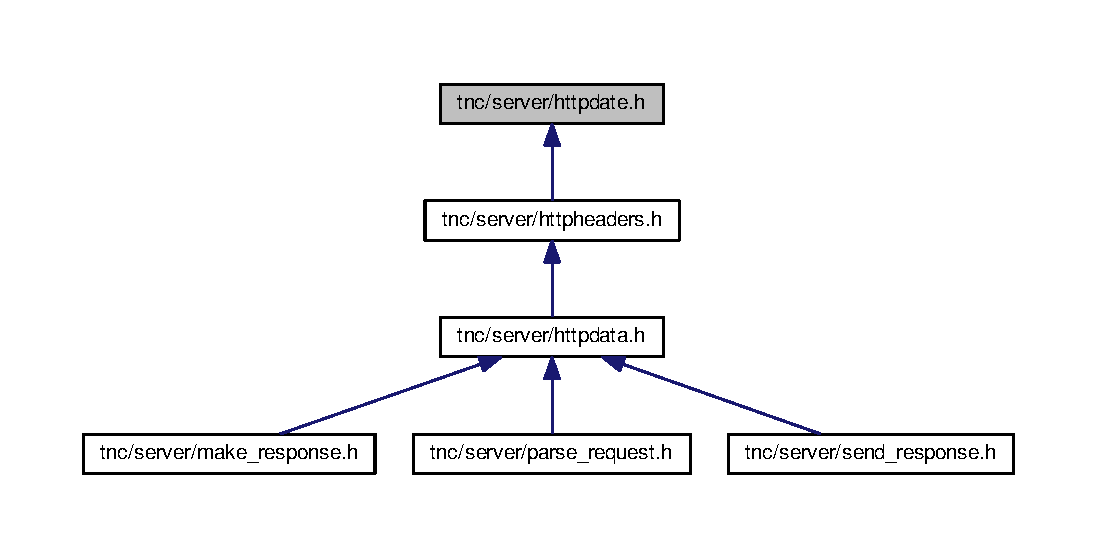
\includegraphics[width=350pt]{httpdate_8h__dep__incl}
\end{center}
\end{figure}
\subsection*{Definizioni}
\begin{Indent}{\bf H\+T\+T\+P\+D\+A\+T\+E}\par
{\em Le definizioni contengono le stringhe in formato leggibile a strptime() rappresentanti le date supportate in ricezione dal server, come indicate dalla R\+F\+C 1945. }\begin{DoxyCompactItemize}
\item 
\hypertarget{httpdate_8h_a619946a84b8848bc8a6e878084b6a2a1}{}\#define {\bfseries H\+T\+T\+P\+D\+A\+T\+E\+\_\+\+R\+F\+C1123}~\char`\"{}\%a, \%d \%b \%Y \%T G\+M\+T\char`\"{}\label{httpdate_8h_a619946a84b8848bc8a6e878084b6a2a1}

\item 
\hypertarget{httpdate_8h_addcfd92b8ccd23beb713242bde512623}{}\#define {\bfseries H\+T\+T\+P\+D\+A\+T\+E\+\_\+\+R\+F\+C850}~\char`\"{}\%A, \%d-\/\%b-\/\%y \%T G\+M\+T\char`\"{}\label{httpdate_8h_addcfd92b8ccd23beb713242bde512623}

\item 
\hypertarget{httpdate_8h_adf2a1b1aba1fc86ab6494bbf7bef6759}{}\#define {\bfseries H\+T\+T\+P\+D\+A\+T\+E\+\_\+\+A\+S\+C\+T\+I\+M\+E}~\char`\"{}\%a \%b \%d \%T \%Y\char`\"{}\label{httpdate_8h_adf2a1b1aba1fc86ab6494bbf7bef6759}

\item 
\hypertarget{httpdate_8h_aca28c4aecc56a5ab016a42296a0ea2ff}{}\#define {\bfseries H\+T\+T\+P\+D\+A\+T\+E}~H\+T\+T\+P\+D\+A\+T\+E\+\_\+\+R\+F\+C1123\label{httpdate_8h_aca28c4aecc56a5ab016a42296a0ea2ff}

\end{DoxyCompactItemize}
\end{Indent}
\subsection*{Funzioni}
\begin{DoxyCompactItemize}
\item 
char $\ast$ \hyperlink{httpdate_8h_a7e14419e90ce1581044f038b5cccb587}{strptime\+\_\+httpdate} (const char $\ast$date, struct tm $\ast$tm)
\begin{DoxyCompactList}\small\item\em Riempie una struct tm a seconda delle informazioni contenute in una stringa. \end{DoxyCompactList}\end{DoxyCompactItemize}


\subsection{Descrizione dettagliata}
Funzioni e definizioni utili alla creazione e alla manipolazione delle date nei formati supportati da H\+T\+T\+P. 



\subsection{Documentazione delle funzioni}
\hypertarget{httpdate_8h_a7e14419e90ce1581044f038b5cccb587}{}\index{httpdate.\+h@{httpdate.\+h}!strptime\+\_\+httpdate@{strptime\+\_\+httpdate}}
\index{strptime\+\_\+httpdate@{strptime\+\_\+httpdate}!httpdate.\+h@{httpdate.\+h}}
\subsubsection[{strptime\+\_\+httpdate}]{\setlength{\rightskip}{0pt plus 5cm}char$\ast$ strptime\+\_\+httpdate (
\begin{DoxyParamCaption}
\item[{const char $\ast$}]{date, }
\item[{struct tm $\ast$}]{tm}
\end{DoxyParamCaption}
)}\label{httpdate_8h_a7e14419e90ce1581044f038b5cccb587}


Riempie una struct tm a seconda delle informazioni contenute in una stringa. 

La funzione si comporta in modo analogo alla funzione P\+O\+S\+I\+X strptime(), ma specificamente per le date H\+T\+T\+P. Il protocollo H\+T\+T\+P/1.\+0 accetta tre diversi formati per la data; la funzione si occupa di scegliere il formato appropriato per la stringa ricevuta come parametro, di eseguire strptime() su di questa e di restituirne il risultato.


\begin{DoxyParams}{Parametri}
{\em date} & La stringa contentente la data di cui fare il parsing.\\
\hline
{\em tm} & La struttura da riempire con le informazioni sulla data.\\
\hline
\end{DoxyParams}
\begin{DoxySeeAlso}{Si veda anche}
strptime() 
\end{DoxySeeAlso}

\hypertarget{httpheaders_8h}{}\section{Riferimenti per il file tnc/server/httpheaders.h}
\label{httpheaders_8h}\index{tnc/server/httpheaders.\+h@{tnc/server/httpheaders.\+h}}


Contiene string literal corrispondenti a header di richiesta e risposta.  


{\ttfamily \#include \char`\"{}httpdate.\+h\char`\"{}}\\*
Grafo delle dipendenze di inclusione per httpheaders.\+h\+:\nopagebreak
\begin{figure}[H]
\begin{center}
\leavevmode
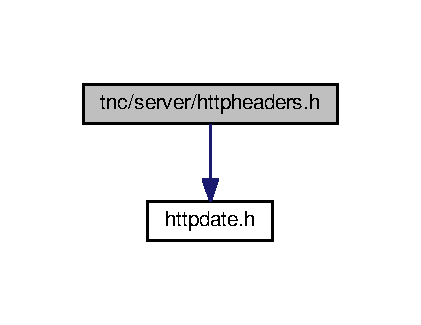
\includegraphics[width=202pt]{httpheaders_8h__incl}
\end{center}
\end{figure}
Questo grafo mostra quali altri file includono direttamente o indirettamente questo file\+:\nopagebreak
\begin{figure}[H]
\begin{center}
\leavevmode
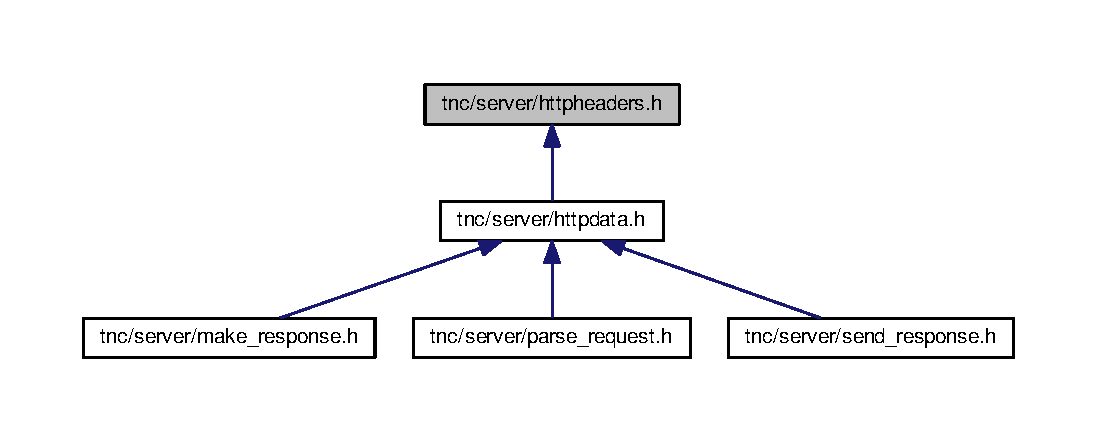
\includegraphics[width=350pt]{httpheaders_8h__dep__incl}
\end{center}
\end{figure}
\subsection*{Definizioni}
\begin{DoxyCompactItemize}
\item 
\hypertarget{httpheaders_8h_aed732fc470f974350bb2b3e6acc81885}{}\#define {\bfseries H\+E\+A\+D\+E\+R\+S\+I\+Z\+E}~8096\label{httpheaders_8h_aed732fc470f974350bb2b3e6acc81885}

\item 
\hypertarget{httpheaders_8h_a6cb23a858b0a21bdaa644b9181dc415f}{}\#define {\bfseries C\+R\+L\+F}~\char`\"{}\textbackslash{}r\textbackslash{}n\char`\"{}\label{httpheaders_8h_a6cb23a858b0a21bdaa644b9181dc415f}

\item 
\hypertarget{httpheaders_8h_a08b924eaac7bce59891b3fbff0eae0c6}{}\#define {\bfseries H\+T\+T\+P10}~\char`\"{}H\+T\+T\+P/1.\+0\char`\"{}\label{httpheaders_8h_a08b924eaac7bce59891b3fbff0eae0c6}

\item 
\hypertarget{httpheaders_8h_aa8e0efb4b744aea5a1a7fcf19949bc34}{}\#define {\bfseries H\+T\+T\+P11}~\char`\"{}H\+T\+T\+P/1.\+1\char`\"{}\label{httpheaders_8h_aa8e0efb4b744aea5a1a7fcf19949bc34}

\item 
\#define \hyperlink{httpheaders_8h_a8d62a6a7cbf8a0a1aa7d13eb0cce2b3a}{C\+O\+M\+M\+A\+N\+D\+\_\+\+M\+I\+M\+E\+T\+Y\+P\+E}~\char`\"{}xdg-\/mime query filetype \%s $\vert$ tr \textquotesingle{}\textbackslash{}\textbackslash{}n\textquotesingle{} \textquotesingle{}\textbackslash{}\textbackslash{}0\textquotesingle{}\char`\"{}
\begin{DoxyCompactList}\small\item\em Comando che viene eseguito per ottenere una stringa contenente il mimetype di un file. \end{DoxyCompactList}\item 
\#define \hyperlink{httpheaders_8h_a5c54332f23fe80ac945f6431b6ca763f}{C\+O\+M\+M\+A\+N\+D\+\_\+\+E\+N\+C\+O\+D\+I\+N\+G}~\char`\"{}file -\/b -\/-\/mime-\/encoding \%s $\vert$ tr \textquotesingle{}\textbackslash{}\textbackslash{}n\textquotesingle{} \textquotesingle{}\textbackslash{}\textbackslash{}0\textquotesingle{}\char`\"{}
\begin{DoxyCompactList}\small\item\em Comando che viene eseguito per ottenere una stringa contenente la codifica di un file. \end{DoxyCompactList}\end{DoxyCompactItemize}
\begin{Indent}{\bf Statusline di risposta}\par
{\em Definizioni di stringhe che rappresentano la statusline di una risposta H\+T\+T\+P. }\begin{DoxyCompactItemize}
\item 
\hypertarget{httpheaders_8h_a52ab6e7e662b67329fe3570d298a09dd}{}\#define {\bfseries R\+H\+D\+R\+\_\+\+S\+T\+A\+T\+U\+S\+L\+I\+N\+E\+\_\+\+O\+K}~\char`\"{}200 O\+K\char`\"{}\label{httpheaders_8h_a52ab6e7e662b67329fe3570d298a09dd}

\item 
\hypertarget{httpheaders_8h_aca5230fd091f852c85521cecf20a7913}{}\#define {\bfseries R\+H\+D\+R\+\_\+\+S\+T\+A\+T\+U\+S\+L\+I\+N\+E\+\_\+\+N\+O\+T\+M\+O\+D\+I\+F\+I\+E\+D}~\char`\"{}304 Not Modified\char`\"{}\label{httpheaders_8h_aca5230fd091f852c85521cecf20a7913}

\item 
\hypertarget{httpheaders_8h_a6870f96252e7a41f53a796fedaf9982f}{}\#define {\bfseries R\+H\+D\+R\+\_\+\+S\+T\+A\+T\+U\+S\+L\+I\+N\+E\+\_\+\+B\+A\+D\+R\+E\+Q\+U\+E\+S\+T}~\char`\"{}400 Bad Request\char`\"{}\label{httpheaders_8h_a6870f96252e7a41f53a796fedaf9982f}

\item 
\hypertarget{httpheaders_8h_a2bfd669aa059c40e7bcb61402462eb84}{}\#define {\bfseries R\+H\+D\+R\+\_\+\+S\+T\+A\+T\+U\+S\+L\+I\+N\+E\+\_\+\+N\+O\+T\+F\+O\+U\+N\+D}~\char`\"{}404 Not Found\char`\"{}\label{httpheaders_8h_a2bfd669aa059c40e7bcb61402462eb84}

\item 
\hypertarget{httpheaders_8h_ae1d88db08dad245759c37ff151ff0f22}{}\#define {\bfseries R\+H\+D\+R\+\_\+\+S\+T\+A\+T\+U\+S\+L\+I\+N\+E\+\_\+\+N\+O\+T\+I\+M\+P\+L\+E\+M\+E\+N\+T\+E\+D}~\char`\"{}501 Not Implemented\char`\"{}\label{httpheaders_8h_ae1d88db08dad245759c37ff151ff0f22}

\end{DoxyCompactItemize}
\end{Indent}
\begin{Indent}{\bf Response header}\par
{\em String literal formattabili con printf() o strfdate() utili alla creazione di una risposta H\+T\+T\+P. }\begin{DoxyCompactItemize}
\item 
\hypertarget{httpheaders_8h_acc0efd1b928f57223437c48dd2407a0f}{}\#define {\bfseries R\+H\+D\+R\+\_\+\+C\+O\+N\+N\+E\+C\+T\+I\+O\+N}~\char`\"{}Connection\+: \%s\char`\"{}\label{httpheaders_8h_acc0efd1b928f57223437c48dd2407a0f}

\item 
\hypertarget{httpheaders_8h_a4c9c30f434da8422e1df4e496738d623}{}\#define {\bfseries R\+H\+D\+R\+\_\+\+C\+O\+N\+T\+E\+N\+T\+\_\+\+T\+Y\+P\+E}~\char`\"{}Content-\/Type\+: \%s; charset=\%s\char`\"{}\label{httpheaders_8h_a4c9c30f434da8422e1df4e496738d623}

\item 
\hypertarget{httpheaders_8h_affac7b401e575c62b6ad921e58aeddbe}{}\#define {\bfseries R\+H\+D\+R\+\_\+\+C\+O\+N\+T\+E\+N\+T\+\_\+\+L\+E\+N\+G\+T\+H}~\char`\"{}Content-\/Length\+: \%s\char`\"{}\label{httpheaders_8h_affac7b401e575c62b6ad921e58aeddbe}

\item 
\hypertarget{httpheaders_8h_a753afe5dd87cbac07c208ca6687d037f}{}\#define {\bfseries R\+H\+D\+R\+\_\+\+L\+A\+S\+T\+\_\+\+M\+O\+D\+I\+F\+I\+E\+D}~\char`\"{}Last-\/Modified\+: \char`\"{} H\+T\+T\+P\+D\+A\+T\+E\label{httpheaders_8h_a753afe5dd87cbac07c208ca6687d037f}

\item 
\hypertarget{httpheaders_8h_ad59b950287aa9c35c83da4db4e475e99}{}\#define {\bfseries R\+H\+D\+R\+\_\+\+D\+A\+T\+E}~\char`\"{}Date\+: \char`\"{} H\+T\+T\+P\+D\+A\+T\+E\label{httpheaders_8h_ad59b950287aa9c35c83da4db4e475e99}

\end{DoxyCompactItemize}
\end{Indent}
\subsection*{Tipi enumerati (enum)}
\begin{DoxyCompactItemize}
\item 
enum \hyperlink{httpheaders_8h_a837a089a977b319a11edfb8022d9e47d}{H\+T\+T\+P\+Method} \{ {\bfseries H\+T\+T\+P\+Method\+\_\+unrecognized}, 
{\bfseries H\+T\+T\+P\+Method\+\_\+\+G\+E\+T}, 
{\bfseries H\+T\+T\+P\+Method\+\_\+\+H\+E\+A\+D}
 \}
\begin{DoxyCompactList}\small\item\em Rappresenta i metodi H\+T\+T\+P riconoscibili ricevuti in ingresso. \end{DoxyCompactList}\end{DoxyCompactItemize}


\subsection{Descrizione dettagliata}
Contiene string literal corrispondenti a header di richiesta e risposta. 



\subsection{Documentazione delle definizioni}
\hypertarget{httpheaders_8h_a5c54332f23fe80ac945f6431b6ca763f}{}\index{httpheaders.\+h@{httpheaders.\+h}!C\+O\+M\+M\+A\+N\+D\+\_\+\+E\+N\+C\+O\+D\+I\+N\+G@{C\+O\+M\+M\+A\+N\+D\+\_\+\+E\+N\+C\+O\+D\+I\+N\+G}}
\index{C\+O\+M\+M\+A\+N\+D\+\_\+\+E\+N\+C\+O\+D\+I\+N\+G@{C\+O\+M\+M\+A\+N\+D\+\_\+\+E\+N\+C\+O\+D\+I\+N\+G}!httpheaders.\+h@{httpheaders.\+h}}
\subsubsection[{C\+O\+M\+M\+A\+N\+D\+\_\+\+E\+N\+C\+O\+D\+I\+N\+G}]{\setlength{\rightskip}{0pt plus 5cm}\#define C\+O\+M\+M\+A\+N\+D\+\_\+\+E\+N\+C\+O\+D\+I\+N\+G~\char`\"{}file -\/b -\/-\/mime-\/encoding \%s $\vert$ tr \textquotesingle{}\textbackslash{}\textbackslash{}n\textquotesingle{} \textquotesingle{}\textbackslash{}\textbackslash{}0\textquotesingle{}\char`\"{}}\label{httpheaders_8h_a5c54332f23fe80ac945f6431b6ca763f}


Comando che viene eseguito per ottenere una stringa contenente la codifica di un file. 

\hypertarget{httpheaders_8h_a8d62a6a7cbf8a0a1aa7d13eb0cce2b3a}{}\index{httpheaders.\+h@{httpheaders.\+h}!C\+O\+M\+M\+A\+N\+D\+\_\+\+M\+I\+M\+E\+T\+Y\+P\+E@{C\+O\+M\+M\+A\+N\+D\+\_\+\+M\+I\+M\+E\+T\+Y\+P\+E}}
\index{C\+O\+M\+M\+A\+N\+D\+\_\+\+M\+I\+M\+E\+T\+Y\+P\+E@{C\+O\+M\+M\+A\+N\+D\+\_\+\+M\+I\+M\+E\+T\+Y\+P\+E}!httpheaders.\+h@{httpheaders.\+h}}
\subsubsection[{C\+O\+M\+M\+A\+N\+D\+\_\+\+M\+I\+M\+E\+T\+Y\+P\+E}]{\setlength{\rightskip}{0pt plus 5cm}\#define C\+O\+M\+M\+A\+N\+D\+\_\+\+M\+I\+M\+E\+T\+Y\+P\+E~\char`\"{}xdg-\/mime query filetype \%s $\vert$ tr \textquotesingle{}\textbackslash{}\textbackslash{}n\textquotesingle{} \textquotesingle{}\textbackslash{}\textbackslash{}0\textquotesingle{}\char`\"{}}\label{httpheaders_8h_a8d62a6a7cbf8a0a1aa7d13eb0cce2b3a}


Comando che viene eseguito per ottenere una stringa contenente il mimetype di un file. 



\subsection{Documentazione dei tipi enumerati}
\hypertarget{httpheaders_8h_a837a089a977b319a11edfb8022d9e47d}{}\index{httpheaders.\+h@{httpheaders.\+h}!H\+T\+T\+P\+Method@{H\+T\+T\+P\+Method}}
\index{H\+T\+T\+P\+Method@{H\+T\+T\+P\+Method}!httpheaders.\+h@{httpheaders.\+h}}
\subsubsection[{H\+T\+T\+P\+Method}]{\setlength{\rightskip}{0pt plus 5cm}enum {\bf H\+T\+T\+P\+Method}}\label{httpheaders_8h_a837a089a977b319a11edfb8022d9e47d}


Rappresenta i metodi H\+T\+T\+P riconoscibili ricevuti in ingresso. 


\hypertarget{make__response_8h}{}\section{Riferimenti per il file tnc/server/make\+\_\+response.h}
\label{make__response_8h}\index{tnc/server/make\+\_\+response.\+h@{tnc/server/make\+\_\+response.\+h}}


Contiene funzioni utili a generare una risposta H\+T\+T\+P.  


{\ttfamily \#include \char`\"{}httpdata.\+h\char`\"{}}\\*
Grafo delle dipendenze di inclusione per make\+\_\+response.\+h\+:\nopagebreak
\begin{figure}[H]
\begin{center}
\leavevmode
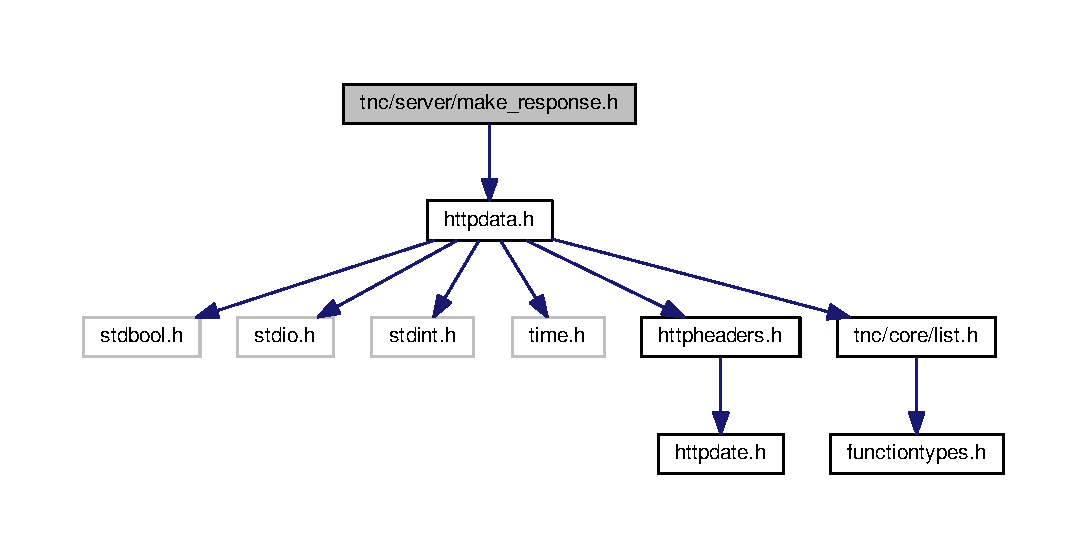
\includegraphics[width=350pt]{make__response_8h__incl}
\end{center}
\end{figure}
\subsection*{Funzioni}
\begin{DoxyCompactItemize}
\item 
\hyperlink{structHTTPResponseData}{H\+T\+T\+P\+Response\+Data} $\ast$ \hyperlink{make__response_8h_adccd9b35824054b0c445e09f0731d706}{make\+\_\+response} (const \hyperlink{structHTTPRequestData}{H\+T\+T\+P\+Request\+Data} $\ast$request\+\_\+data)
\begin{DoxyCompactList}\small\item\em Data una richiesta, restituisce un \hyperlink{structHTTPResponseData}{H\+T\+T\+P\+Response\+Data} contenente gli elementi necessari a generare una risposta. \end{DoxyCompactList}\end{DoxyCompactItemize}


\subsection{Descrizione dettagliata}
Contiene funzioni utili a generare una risposta H\+T\+T\+P. 



\subsection{Documentazione delle funzioni}
\hypertarget{make__response_8h_adccd9b35824054b0c445e09f0731d706}{}\index{make\+\_\+response.\+h@{make\+\_\+response.\+h}!make\+\_\+response@{make\+\_\+response}}
\index{make\+\_\+response@{make\+\_\+response}!make\+\_\+response.\+h@{make\+\_\+response.\+h}}
\subsubsection[{make\+\_\+response}]{\setlength{\rightskip}{0pt plus 5cm}{\bf H\+T\+T\+P\+Response\+Data}$\ast$ make\+\_\+response (
\begin{DoxyParamCaption}
\item[{const {\bf H\+T\+T\+P\+Request\+Data} $\ast$}]{request\+\_\+data}
\end{DoxyParamCaption}
)}\label{make__response_8h_adccd9b35824054b0c445e09f0731d706}


Data una richiesta, restituisce un \hyperlink{structHTTPResponseData}{H\+T\+T\+P\+Response\+Data} contenente gli elementi necessari a generare una risposta. 


\begin{DoxyParams}{Parametri}
{\em request\+\_\+data} & L\textquotesingle{}\hyperlink{structHTTPRequestData}{H\+T\+T\+P\+Request\+Data} per cui si vuole generare una risposta.\\
\hline
\end{DoxyParams}
\begin{DoxyReturn}{Restituisce}
Un \hyperlink{structHTTPResponseData}{H\+T\+T\+P\+Response\+Data} contenente gli header e i file descriptor utili all\textquotesingle{}invio della risposta.
\end{DoxyReturn}
\begin{DoxySeeAlso}{Si veda anche}
\hyperlink{structHTTPResponseData}{H\+T\+T\+P\+Response\+Data} 
\end{DoxySeeAlso}

\hypertarget{parse__request_8h}{}\section{Riferimenti per il file tnc/server/parse\+\_\+request.h}
\label{parse__request_8h}\index{tnc/server/parse\+\_\+request.\+h@{tnc/server/parse\+\_\+request.\+h}}


Contiene elementi utili al parsing della richiesta H\+T\+T\+P.  


{\ttfamily \#include \char`\"{}httpdata.\+h\char`\"{}}\\*
Grafo delle dipendenze di inclusione per parse\+\_\+request.\+h\+:\nopagebreak
\begin{figure}[H]
\begin{center}
\leavevmode
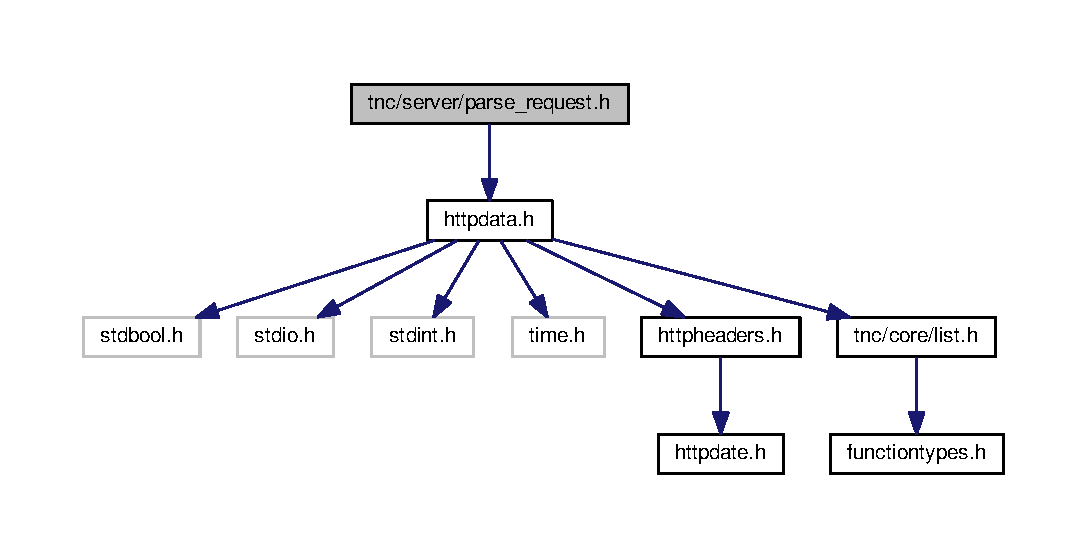
\includegraphics[width=350pt]{parse__request_8h__incl}
\end{center}
\end{figure}
\subsection*{Funzioni}
\begin{DoxyCompactItemize}
\item 
\hyperlink{structHTTPRequestData}{H\+T\+T\+P\+Request\+Data} $\ast$ \hyperlink{parse__request_8h_a7f6b46b8f33ebe0426d0d13b320f2927}{parse\+\_\+request} (T\+N\+C\+Server self, char $\ast$request)
\begin{DoxyCompactList}\small\item\em Data una richiesta e il server che la riceve, restituisce un puntatore a un \hyperlink{structHTTPRequestData}{H\+T\+T\+P\+Request\+Data} contenente informazioni su di questa. \end{DoxyCompactList}\end{DoxyCompactItemize}


\subsection{Descrizione dettagliata}
Contiene elementi utili al parsing della richiesta H\+T\+T\+P. 



\subsection{Documentazione delle funzioni}
\hypertarget{parse__request_8h_a7f6b46b8f33ebe0426d0d13b320f2927}{}\index{parse\+\_\+request.\+h@{parse\+\_\+request.\+h}!parse\+\_\+request@{parse\+\_\+request}}
\index{parse\+\_\+request@{parse\+\_\+request}!parse\+\_\+request.\+h@{parse\+\_\+request.\+h}}
\subsubsection[{parse\+\_\+request}]{\setlength{\rightskip}{0pt plus 5cm}{\bf H\+T\+T\+P\+Request\+Data}$\ast$ parse\+\_\+request (
\begin{DoxyParamCaption}
\item[{T\+N\+C\+Server}]{self, }
\item[{char $\ast$}]{request}
\end{DoxyParamCaption}
)}\label{parse__request_8h_a7f6b46b8f33ebe0426d0d13b320f2927}


Data una richiesta e il server che la riceve, restituisce un puntatore a un \hyperlink{structHTTPRequestData}{H\+T\+T\+P\+Request\+Data} contenente informazioni su di questa. 


\begin{DoxyParams}{Parametri}
{\em request} & La stringa contenente la richiesta H\+T\+T\+P.\\
\hline
{\em self} & Il server su cui si sta operando.\\
\hline
\end{DoxyParams}
\begin{DoxyReturn}{Restituisce}
Un puntatore a un \hyperlink{structHTTPRequestData}{H\+T\+T\+P\+Request\+Data} contenente informazioni sulla richiesta.
\end{DoxyReturn}
\begin{DoxySeeAlso}{Si veda anche}
\hyperlink{structHTTPRequestData}{H\+T\+T\+P\+Request\+Data} 
\end{DoxySeeAlso}

\hypertarget{paths_8h}{}\section{Riferimenti per il file tnc/server/paths.h}
\label{paths_8h}\index{tnc/server/paths.\+h@{tnc/server/paths.\+h}}


Contiene definizioni e funzioni utili nell\textquotesingle{}ambito dell\textquotesingle{}elaborazione dei percorsi.  


{\ttfamily \#include $<$stdio.\+h$>$}\\*
{\ttfamily \#include \char`\"{}server.\+h\char`\"{}}\\*
Grafo delle dipendenze di inclusione per paths.\+h\+:
\nopagebreak
\begin{figure}[H]
\begin{center}
\leavevmode
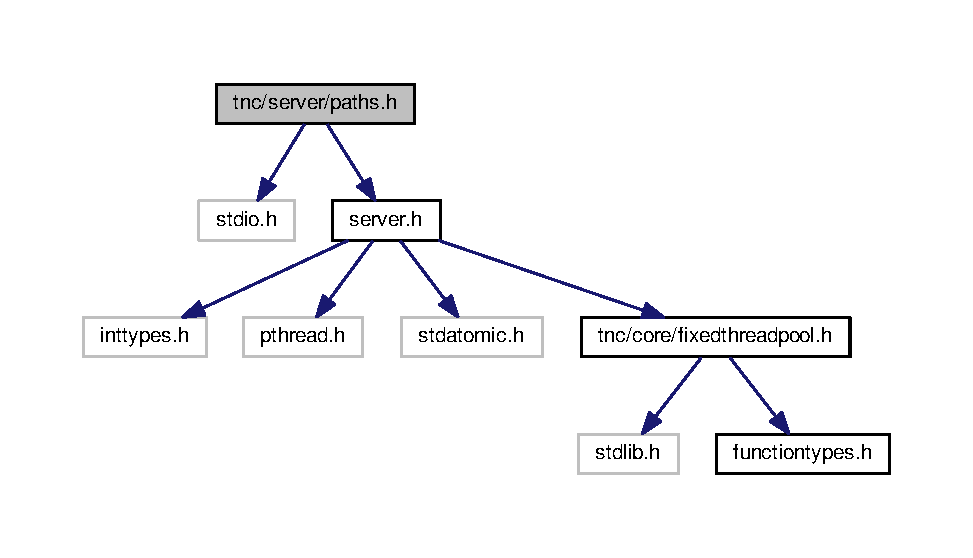
\includegraphics[width=350pt]{paths_8h__incl}
\end{center}
\end{figure}
\subsection*{Definizioni}
\begin{DoxyCompactItemize}
\item 
\hypertarget{paths_8h_a746109abf85b0689cd68472143a17195}{}\#define {\bfseries P\+A\+T\+H\+\_\+\+R\+O\+O\+T}~\char`\"{}/\char`\"{}\label{paths_8h_a746109abf85b0689cd68472143a17195}

\item 
\hypertarget{paths_8h_ae95b6c5c06561e0e56702a4475f82800}{}\#define {\bfseries P\+A\+T\+H\+\_\+\+I\+N\+D\+E\+X\+H\+T\+M}~\char`\"{}/index.\+htm\char`\"{}\label{paths_8h_ae95b6c5c06561e0e56702a4475f82800}

\item 
\hypertarget{paths_8h_ac73cdc58e693a2bc1e1e6f4d0b36606c}{}\#define {\bfseries P\+A\+T\+H\+\_\+\+I\+N\+D\+E\+X\+H\+T\+M\+L}~\char`\"{}/index.\+html\char`\"{}\label{paths_8h_ac73cdc58e693a2bc1e1e6f4d0b36606c}

\item 
\hypertarget{paths_8h_a018b9d974ad0af4120f2b9c3b290a540}{}\#define {\bfseries P\+A\+T\+H\+\_\+\+D\+E\+F\+A\+U\+L\+T\+\_\+\+E\+R\+R\+O\+R}~\char`\"{}./pages/\%i.\+html\char`\"{}\label{paths_8h_a018b9d974ad0af4120f2b9c3b290a540}

\end{DoxyCompactItemize}
\subsection*{Funzioni}
\begin{DoxyCompactItemize}
\item 
char $\ast$ \hyperlink{paths_8h_a745b3acac88175c54e73a10273f95709}{get\+\_\+index\+\_\+path} (T\+N\+C\+Server self)
\begin{DoxyCompactList}\small\item\em Dato un server, restituisce il percorso del file index della cartella che serve. \end{DoxyCompactList}\end{DoxyCompactItemize}


\subsection{Descrizione dettagliata}
Contiene definizioni e funzioni utili nell\textquotesingle{}ambito dell\textquotesingle{}elaborazione dei percorsi. 



\subsection{Documentazione delle funzioni}
\hypertarget{paths_8h_a745b3acac88175c54e73a10273f95709}{}\index{paths.\+h@{paths.\+h}!get\+\_\+index\+\_\+path@{get\+\_\+index\+\_\+path}}
\index{get\+\_\+index\+\_\+path@{get\+\_\+index\+\_\+path}!paths.\+h@{paths.\+h}}
\subsubsection[{get\+\_\+index\+\_\+path}]{\setlength{\rightskip}{0pt plus 5cm}char$\ast$ get\+\_\+index\+\_\+path (
\begin{DoxyParamCaption}
\item[{T\+N\+C\+Server}]{self}
\end{DoxyParamCaption}
)}\label{paths_8h_a745b3acac88175c54e73a10273f95709}


Dato un server, restituisce il percorso del file index della cartella che serve. 


\begin{DoxyParams}{Parametri}
{\em self} & Il server di riferimento.\\
\hline
\end{DoxyParams}
\begin{DoxyReturn}{Restituisce}
Il percorso di un file index.\+htm o index.\+html nella cartella che il server sta servendo. Se non ce n\textquotesingle{}è uno, N\+U\+L\+L. 
\end{DoxyReturn}

\hypertarget{send__response_8h}{}\section{Riferimenti per il file tnc/server/send\+\_\+response.h}
\label{send__response_8h}\index{tnc/server/send\+\_\+response.\+h@{tnc/server/send\+\_\+response.\+h}}


Contiene definizioni e funzioni utili all\textquotesingle{}invio di risposte H\+T\+T\+P.  


{\ttfamily \#include $<$stdbool.\+h$>$}\\*
{\ttfamily \#include \char`\"{}httpdata.\+h\char`\"{}}\\*
Grafo delle dipendenze di inclusione per send\+\_\+response.\+h\+:\nopagebreak
\begin{figure}[H]
\begin{center}
\leavevmode
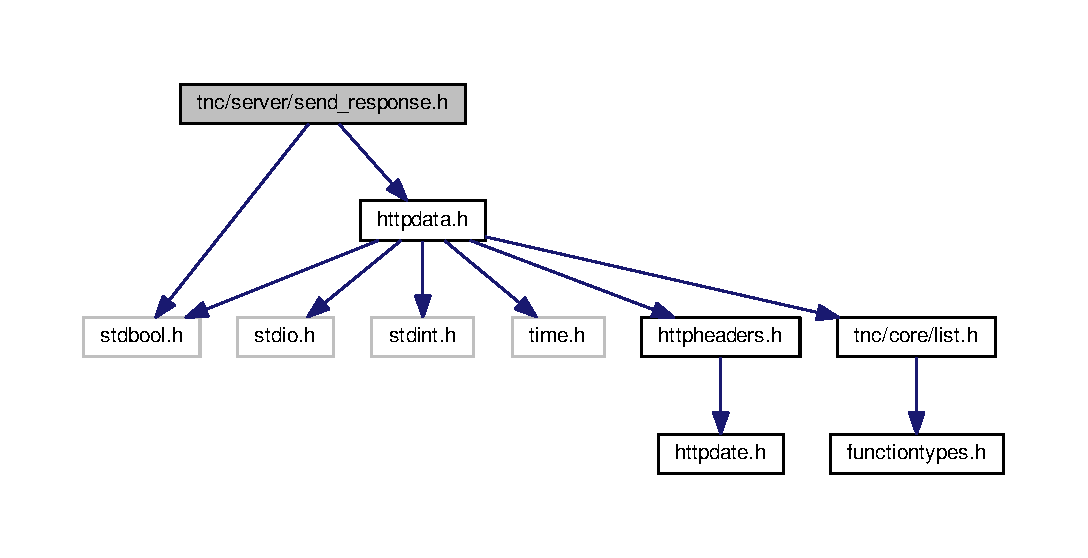
\includegraphics[width=350pt]{send__response_8h__incl}
\end{center}
\end{figure}
\subsection*{Funzioni}
\begin{DoxyCompactItemize}
\item 
bool \hyperlink{send__response_8h_aee7d986f80a17267af7a83aac0a1ed74}{send\+\_\+response} (int connection\+\_\+socket, \hyperlink{structHTTPResponseData}{H\+T\+T\+P\+Response\+Data} $\ast$data)
\begin{DoxyCompactList}\small\item\em Invia una risposta tramite un socket. \end{DoxyCompactList}\end{DoxyCompactItemize}


\subsection{Descrizione dettagliata}
Contiene definizioni e funzioni utili all\textquotesingle{}invio di risposte H\+T\+T\+P. 



\subsection{Documentazione delle funzioni}
\hypertarget{send__response_8h_aee7d986f80a17267af7a83aac0a1ed74}{}\index{send\+\_\+response.\+h@{send\+\_\+response.\+h}!send\+\_\+response@{send\+\_\+response}}
\index{send\+\_\+response@{send\+\_\+response}!send\+\_\+response.\+h@{send\+\_\+response.\+h}}
\subsubsection[{send\+\_\+response}]{\setlength{\rightskip}{0pt plus 5cm}bool send\+\_\+response (
\begin{DoxyParamCaption}
\item[{int}]{connection\+\_\+socket, }
\item[{{\bf H\+T\+T\+P\+Response\+Data} $\ast$}]{data}
\end{DoxyParamCaption}
)}\label{send__response_8h_aee7d986f80a17267af7a83aac0a1ed74}


Invia una risposta tramite un socket. 

La funzione invia tramite connection\+\_\+socket una risposta H\+T\+T\+P, composta dagli header e dal file contenuti in data. Per comporre il parametro data, usare \hyperlink{make__response_8h_adccd9b35824054b0c445e09f0731d706}{make\+\_\+response()}.


\begin{DoxyParams}{Parametri}
{\em connection\+\_\+socket} & Il socket attraverso cui inviare la risposta.\\
\hline
{\em data} & I dati sulla risposta da inviare.\\
\hline
\end{DoxyParams}
\begin{DoxyReturn}{Restituisce}
L\textquotesingle{}esito dell\textquotesingle{}operazione, true se è andata a buon fine, false altrimenti.$\ast$ 
\end{DoxyReturn}

\hypertarget{server_8h}{}\section{Riferimenti per il file tnc/server/server.h}
\label{server_8h}\index{tnc/server/server.\+h@{tnc/server/server.\+h}}


Contiene funzioni utili all\textquotesingle{}uso del server.  


{\ttfamily \#include $<$inttypes.\+h$>$}\\*
{\ttfamily \#include $<$pthread.\+h$>$}\\*
{\ttfamily \#include $<$stdatomic.\+h$>$}\\*
{\ttfamily \#include \char`\"{}tnc/core/fixedthreadpool.\+h\char`\"{}}\\*
Grafo delle dipendenze di inclusione per server.\+h\+:
\nopagebreak
\begin{figure}[H]
\begin{center}
\leavevmode
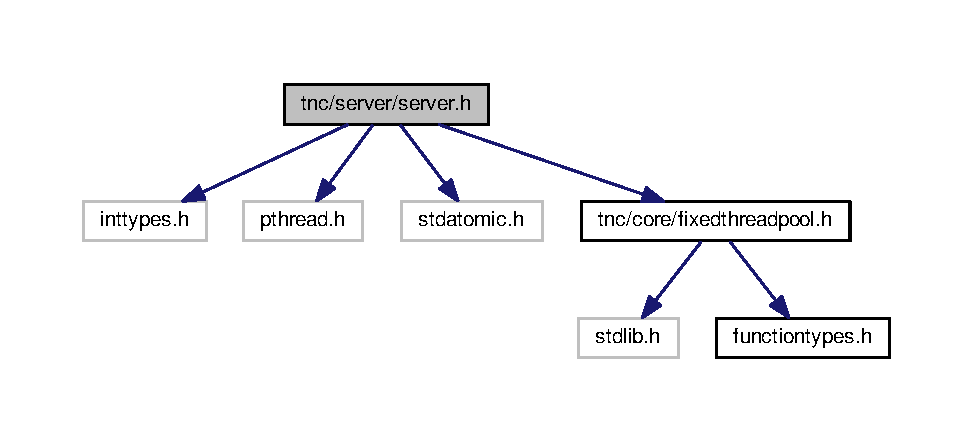
\includegraphics[width=350pt]{server_8h__incl}
\end{center}
\end{figure}
Questo grafo mostra quali altri file includono direttamente o indirettamente questo file\+:
\nopagebreak
\begin{figure}[H]
\begin{center}
\leavevmode
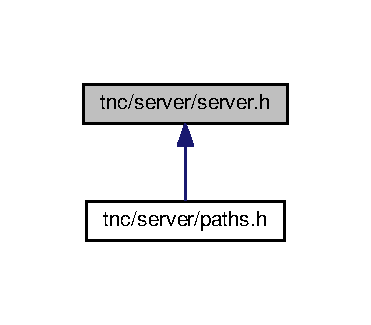
\includegraphics[width=178pt]{server_8h__dep__incl}
\end{center}
\end{figure}
\subsection*{Tipi enumerati (enum)}
\begin{DoxyCompactItemize}
\item 
\hypertarget{server_8h_a0249264e0c8e46746c777adca61d5947}{}enum {\bfseries T\+N\+C\+Server\+\_\+shutdown} \{ {\bfseries T\+N\+C\+Server\+\_\+shutdown\+\_\+now} = T\+N\+C\+Thread\+Pool\+\_\+shutdown\+\_\+now, 
{\bfseries T\+N\+C\+Server\+\_\+shutdown\+\_\+finish\+\_\+pending} = T\+N\+C\+Thread\+Pool\+\_\+shutdown\+\_\+finish\+\_\+pending
 \}\label{server_8h_a0249264e0c8e46746c777adca61d5947}

\item 
\hypertarget{server_8h_acef63214d9d61a268fa7b96ce5b353da}{}enum {\bfseries T\+N\+C\+Server\+\_\+wait} \{ {\bfseries T\+N\+C\+Server\+\_\+wait\+\_\+yes} = T\+N\+C\+Thread\+Pool\+\_\+wait\+\_\+yes, 
{\bfseries T\+N\+C\+Server\+\_\+wait\+\_\+no} = T\+N\+C\+Thread\+Pool\+\_\+wait\+\_\+no
 \}\label{server_8h_acef63214d9d61a268fa7b96ce5b353da}

\end{DoxyCompactItemize}
\subsection*{Funzioni}
\begin{DoxyCompactItemize}
\item 
T\+N\+C\+Server \hyperlink{server_8h_aae87182289b15731e1abbe5469d2e90a}{T\+N\+C\+Server\+\_\+new} (const char $\ast$localpath, uint16\+\_\+t door, size\+\_\+t max\+\_\+threads)
\begin{DoxyCompactList}\small\item\em Crea un nuovo T\+N\+C\+Server. \end{DoxyCompactList}\item 
int \hyperlink{server_8h_ada04abafbddbfd9bc5e02c50334ecc55}{T\+N\+C\+Server\+\_\+start} (T\+N\+C\+Server self)
\begin{DoxyCompactList}\small\item\em Avvia il T\+N\+C\+Server passato come parametro, ovvero inizia ad ascoltare e a rispondere alle richieste che riceve. \end{DoxyCompactList}\item 
void \hyperlink{server_8h_a54908b6bb01370749a3105d45d5bad90}{T\+N\+C\+Server\+\_\+shutdown} (T\+N\+C\+Server self, enum T\+N\+C\+Server\+\_\+shutdown shutdown, enum T\+N\+C\+Server\+\_\+wait wait)
\begin{DoxyCompactList}\small\item\em Termina il T\+N\+C\+Server passato come parametro. \end{DoxyCompactList}\item 
void \hyperlink{server_8h_ab67b044525ad306fe48ae6974e2cd74c}{T\+N\+C\+Server\+\_\+destroy} (T\+N\+C\+Server self)
\begin{DoxyCompactList}\small\item\em Elimina (dealloca) un T\+N\+C\+Server. \end{DoxyCompactList}\end{DoxyCompactItemize}


\subsection{Descrizione dettagliata}
Contiene funzioni utili all\textquotesingle{}uso del server. 



\subsection{Documentazione delle funzioni}
\hypertarget{server_8h_ab67b044525ad306fe48ae6974e2cd74c}{}\index{server.\+h@{server.\+h}!T\+N\+C\+Server\+\_\+destroy@{T\+N\+C\+Server\+\_\+destroy}}
\index{T\+N\+C\+Server\+\_\+destroy@{T\+N\+C\+Server\+\_\+destroy}!server.\+h@{server.\+h}}
\subsubsection[{T\+N\+C\+Server\+\_\+destroy}]{\setlength{\rightskip}{0pt plus 5cm}void T\+N\+C\+Server\+\_\+destroy (
\begin{DoxyParamCaption}
\item[{T\+N\+C\+Server}]{self}
\end{DoxyParamCaption}
)}\label{server_8h_ab67b044525ad306fe48ae6974e2cd74c}


Elimina (dealloca) un T\+N\+C\+Server. 

\hypertarget{server_8h_aae87182289b15731e1abbe5469d2e90a}{}\index{server.\+h@{server.\+h}!T\+N\+C\+Server\+\_\+new@{T\+N\+C\+Server\+\_\+new}}
\index{T\+N\+C\+Server\+\_\+new@{T\+N\+C\+Server\+\_\+new}!server.\+h@{server.\+h}}
\subsubsection[{T\+N\+C\+Server\+\_\+new}]{\setlength{\rightskip}{0pt plus 5cm}T\+N\+C\+Server T\+N\+C\+Server\+\_\+new (
\begin{DoxyParamCaption}
\item[{const char $\ast$}]{localpath, }
\item[{uint16\+\_\+t}]{door, }
\item[{size\+\_\+t}]{max\+\_\+threads}
\end{DoxyParamCaption}
)}\label{server_8h_aae87182289b15731e1abbe5469d2e90a}


Crea un nuovo T\+N\+C\+Server. 


\begin{DoxyParams}{Parametri}
{\em localpath} & Il percorso locale da servire.\\
\hline
{\em door} & La porta su cui il server deve operare.\\
\hline
{\em max\+\_\+threads} & Il numero massimo di thread che il server può usare.\\
\hline
\end{DoxyParams}
\begin{DoxyReturn}{Restituisce}
Un puntatore opaco a un T\+N\+C\+Server. 
\end{DoxyReturn}
\hypertarget{server_8h_a54908b6bb01370749a3105d45d5bad90}{}\index{server.\+h@{server.\+h}!T\+N\+C\+Server\+\_\+shutdown@{T\+N\+C\+Server\+\_\+shutdown}}
\index{T\+N\+C\+Server\+\_\+shutdown@{T\+N\+C\+Server\+\_\+shutdown}!server.\+h@{server.\+h}}
\subsubsection[{T\+N\+C\+Server\+\_\+shutdown}]{\setlength{\rightskip}{0pt plus 5cm}void T\+N\+C\+Server\+\_\+shutdown (
\begin{DoxyParamCaption}
\item[{T\+N\+C\+Server}]{self, }
\item[{enum T\+N\+C\+Server\+\_\+shutdown}]{shutdown, }
\item[{enum T\+N\+C\+Server\+\_\+wait}]{wait}
\end{DoxyParamCaption}
)}\label{server_8h_a54908b6bb01370749a3105d45d5bad90}


Termina il T\+N\+C\+Server passato come parametro. 


\begin{DoxyParams}{Parametri}
{\em self} & Il server su cui si vuole operare.\\
\hline
{\em shutdown} & Se settato su T\+N\+C\+Server\+\_\+shutdown\+\_\+finish\+\_\+pending, viene attesa l\textquotesingle{}elaborazione delle richieste già ricevute dal server prima di terminarlo. Se settato su T\+N\+C\+Server\+\_\+shutdown\+\_\+now, il server esegue l\textquotesingle{}elaborazione delle sole richieste su cui ha già iniziato ad operare prima di terminare.\\
\hline
{\em wait} & Se settato su T\+N\+C\+Server\+\_\+wait\+\_\+yes, la funzione attende la terminazione del server prima di terminare. Se settato su T\+N\+C\+Server\+\_\+wait\+\_\+no, la chiamata a T\+N\+C\+Server\+\_\+shutdown termina immediatamente. \\
\hline
\end{DoxyParams}
\hypertarget{server_8h_ada04abafbddbfd9bc5e02c50334ecc55}{}\index{server.\+h@{server.\+h}!T\+N\+C\+Server\+\_\+start@{T\+N\+C\+Server\+\_\+start}}
\index{T\+N\+C\+Server\+\_\+start@{T\+N\+C\+Server\+\_\+start}!server.\+h@{server.\+h}}
\subsubsection[{T\+N\+C\+Server\+\_\+start}]{\setlength{\rightskip}{0pt plus 5cm}int T\+N\+C\+Server\+\_\+start (
\begin{DoxyParamCaption}
\item[{T\+N\+C\+Server}]{self}
\end{DoxyParamCaption}
)}\label{server_8h_ada04abafbddbfd9bc5e02c50334ecc55}


Avvia il T\+N\+C\+Server passato come parametro, ovvero inizia ad ascoltare e a rispondere alle richieste che riceve. 


\begin{DoxyParams}{Parametri}
{\em self} & Il server da avviare.\\
\hline
\end{DoxyParams}
\begin{DoxyReturn}{Restituisce}
0 se va a buon fine, un codice di errore altrimenti. I codici di errore relativi al server possono essere consultati nell\textquotesingle{}header \hyperlink{server_2error_8h}{tnc/server/error.\+h}
\end{DoxyReturn}
\begin{DoxySeeAlso}{Si veda anche}
error.\+h 
\end{DoxySeeAlso}

%--- End generated contents ---

% Index
\backmatter
\newpage
\phantomsection
\clearemptydoublepage
\addcontentsline{toc}{chapter}{Indice}
\printindex

\end{document}
